%!TEX root = ../../super_main.tex

\section{Participant Interaction}
When opening the mobile application, the participant is presented with an initial, as seen in \figref{fig:initial_screen}. The idea with this screen is to welcome the participant to the application. Currently, it does not supply the participant with much information, but one could imagine that this view would, in future iterations, provide the participant with usable information, such as progress in the current campaign, clarification of what concepts and principals the participants must know. This screen could possibly also contain some motivational factor, provided by customers. e.g. a ``prize'' for participation.

\todo[inline]{Skriv at vi bruger Google Material Design som udgangspunkt. Så har vi nogle ``standard'' elementer og principper at gå ud fra, så vi slipper for at opfinde den dybe tallerken}

\todo[inline]{Skriv at vi igennem sektionen også viser vores mockups/initial design af de forskellige views.}

% Initial screen
\begin{figure}[!htbp]
\begin{subfigure}[!t]{.48\textwidth}
  \centering
  
\includegraphics[width=.7\linewidth]{mockups/homepage}
  \caption{Mockup.}
  \label{fig:mockup_initial_screen}
\end{subfigure}%
\begin{subfigure}[!t]{.52\textwidth}
  \centering
  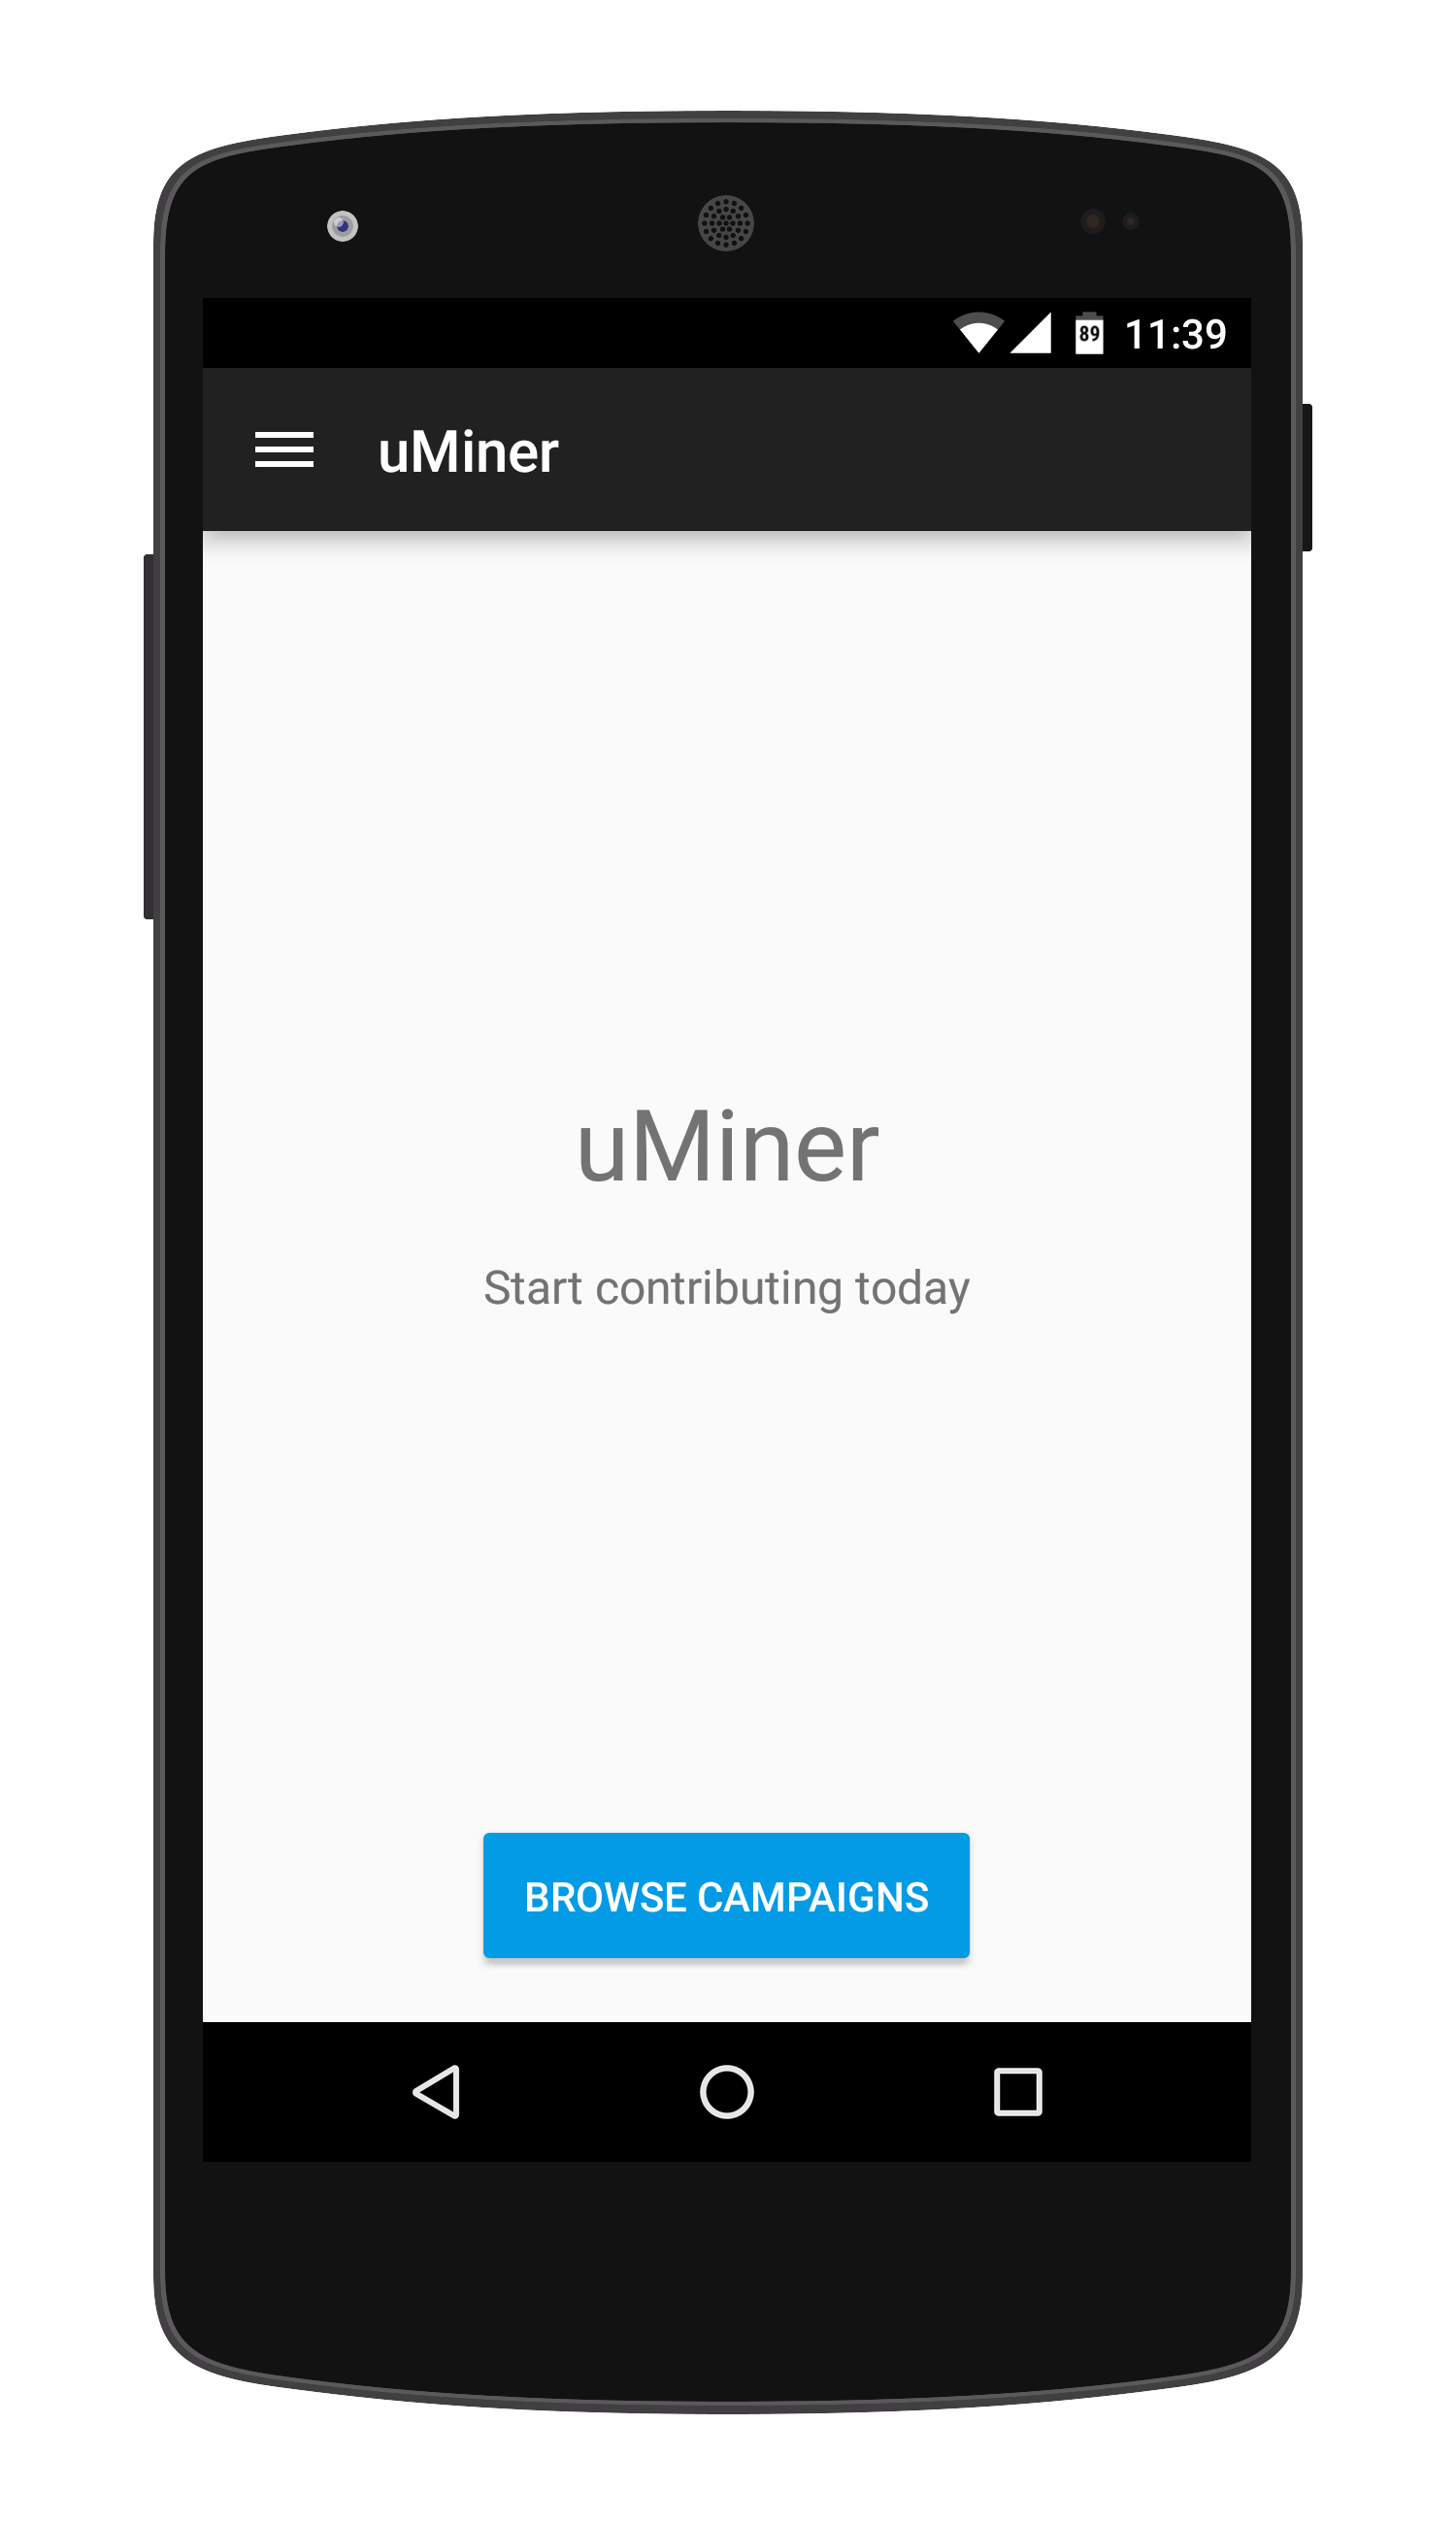
\includegraphics[width=.73\linewidth]{user_interfaces/client/client_uminer_home_with_phone}
  \caption{Implementation.}
  \label{fig:implementation_initial_screen}
\end{subfigure}
\caption{Initial screen of the Application.}
\label{fig:initial_screen}
\end{figure}
\FloatBarrier

To navigate to other views in the application, the participants must either use the drawer menu displayed in \figref{fig:navigation} or the \emph{browse campaigns}-button in the initial view. The navigation menu contains three elements, which will each take the participant to different parts of the application.

\begin{description}
	\item[``Current campaign''] redirects the participant to a campaign specification view, as seen in \figref{fig:specific_campaign}, displaying more information about the campaign that they are currently contributing to. If the participant have not yet joined a campaign, a message will briefly be displayed on the screen, informing the participant about this.

	\item[``Browse campaigns''] redirects the participant to a view containing brief information about all of the publicly available campaigns, as seen in \figref{fig:public_campaigns}.

	\item[``Join specific''] redirects the participant to a view, as seen in \figref{fig:specific_campaign}, where he/she can search for a specific campaign by providing a campaign identifier.
\end{description}

% Navigation
\begin{figure}[!htbp]
\centering
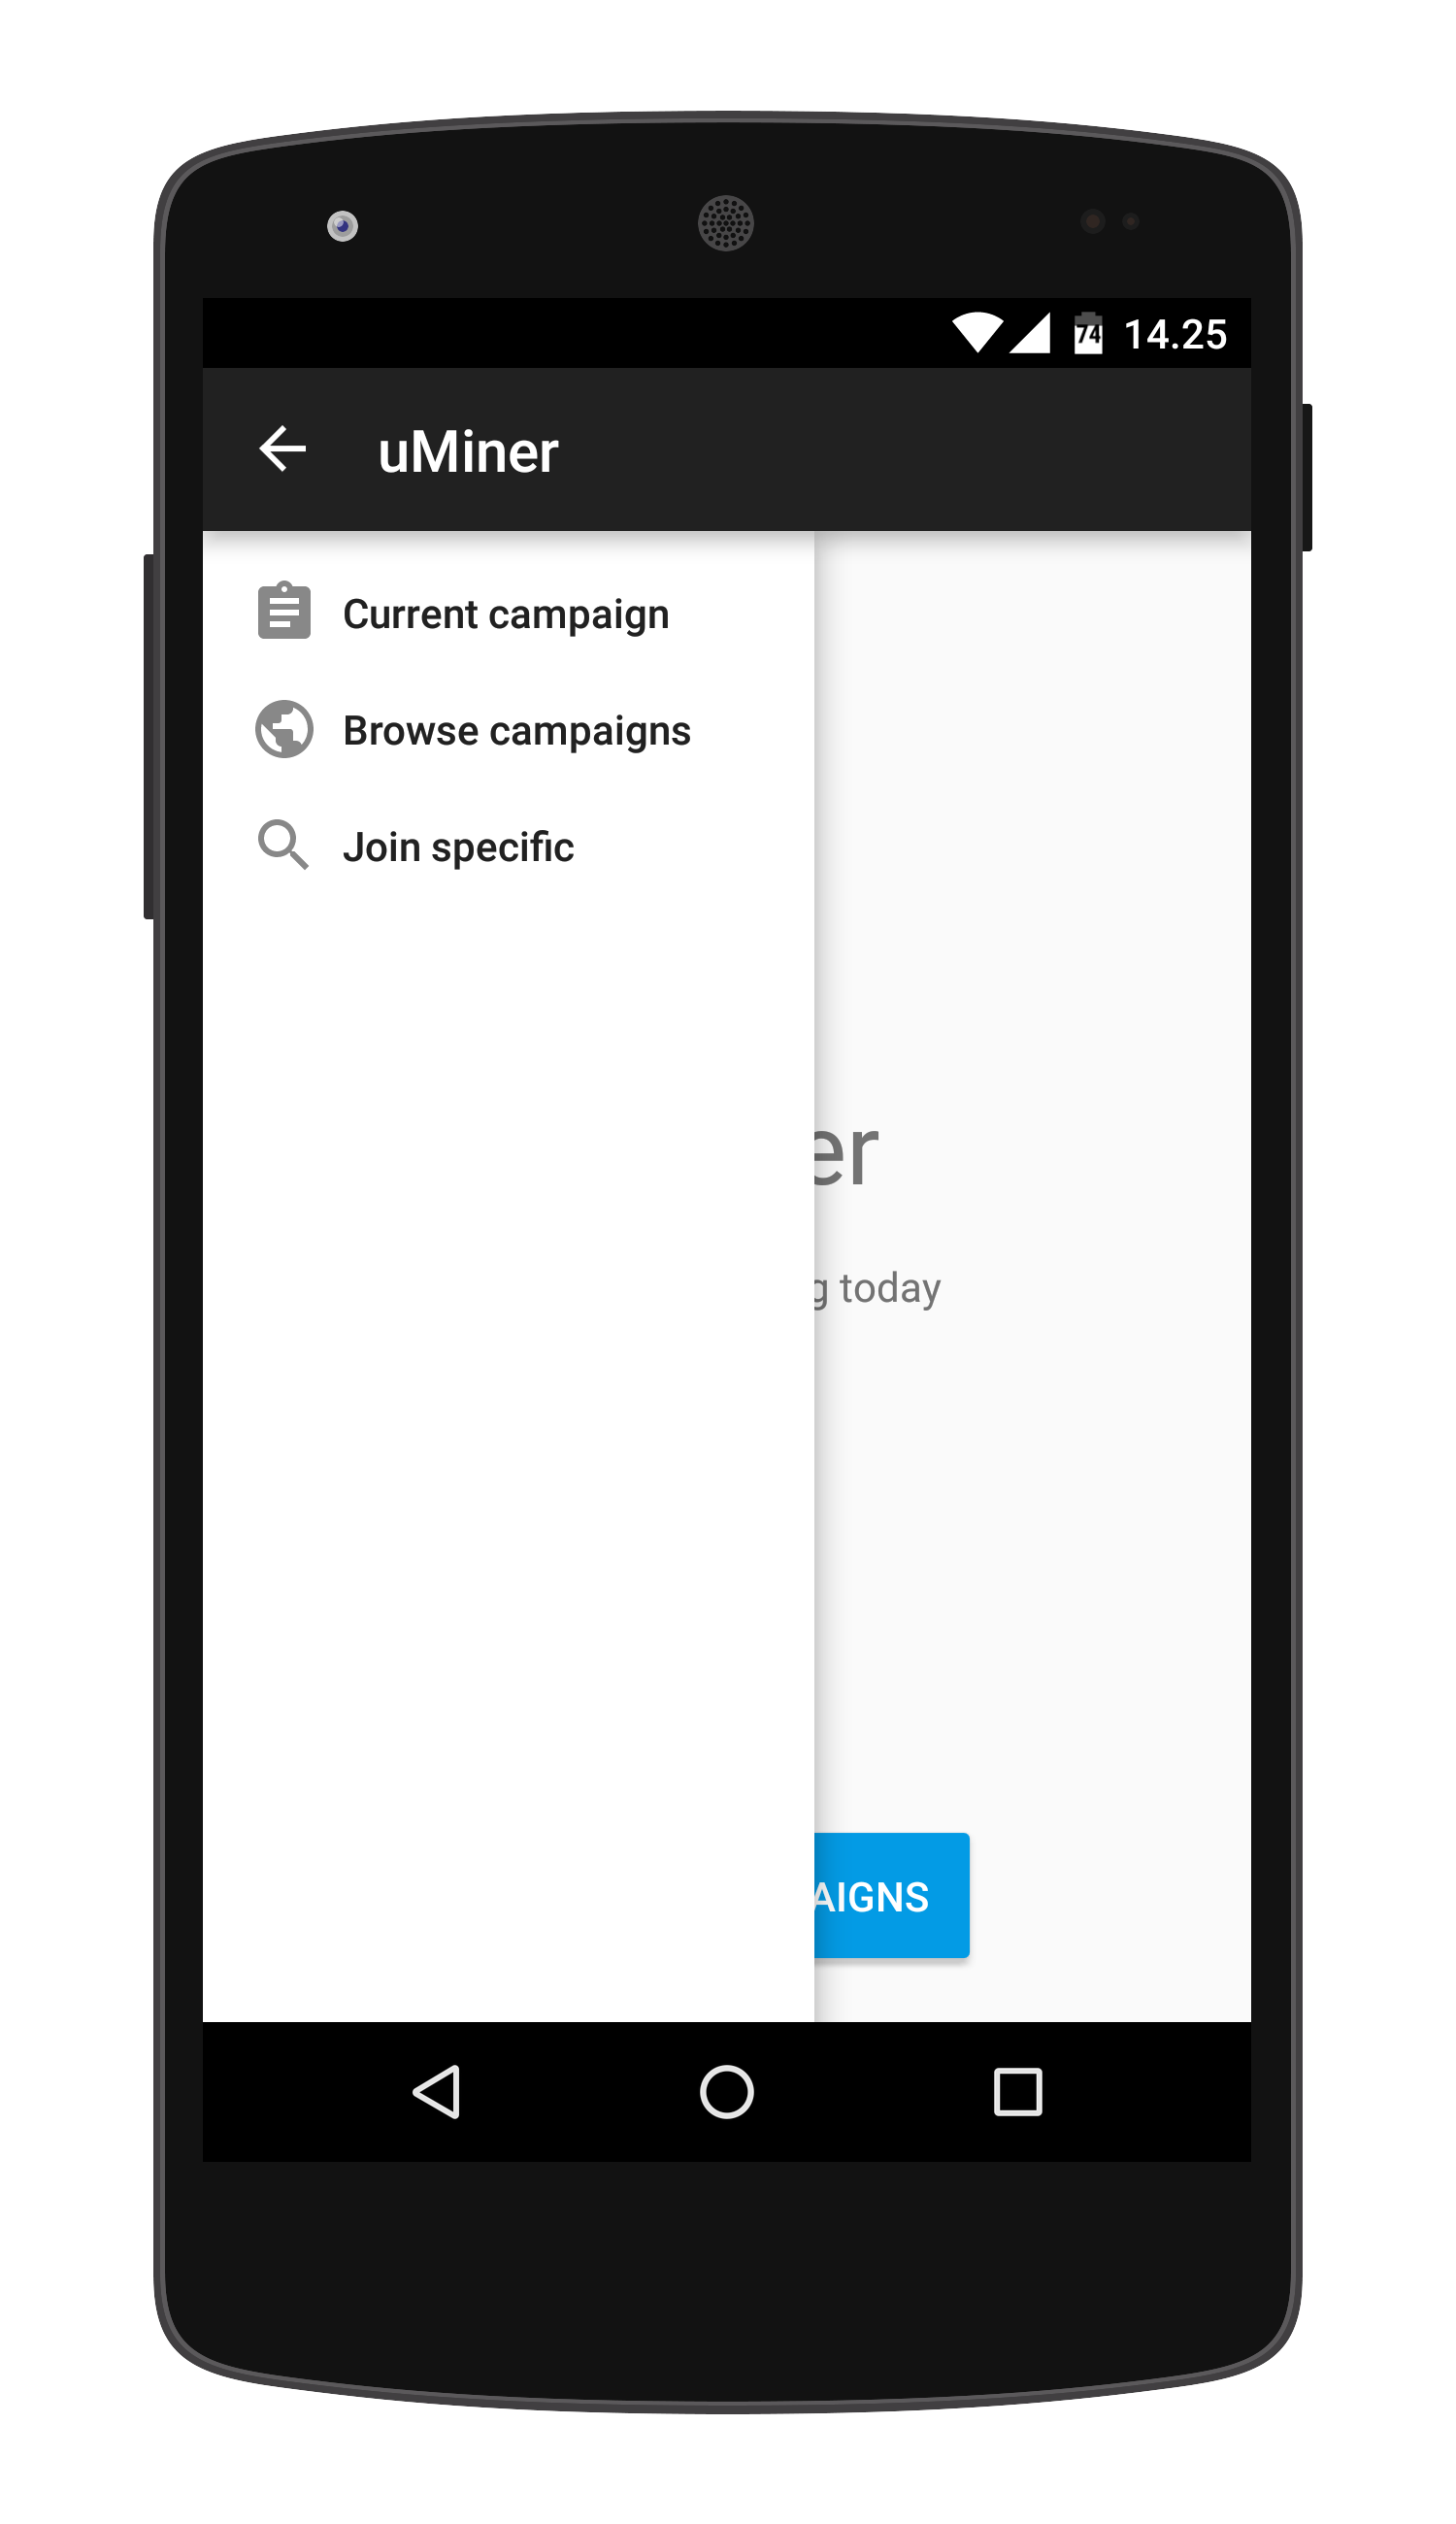
\includegraphics[width=.35\linewidth]{user_interfaces/client/client_drawer_menu_with_phone}
\caption{Navigation through the application.}
\label{fig:navigation}
\end{figure}
\FloatBarrier

\subsection{Browsing Campaigns}
If a participant wants to contribute to a campaign, they may browse the publicly available campaigns. This can be done through the view seen in \figref{fig:public_campaigns}. Here, all campaigns are listed displaying the title of the campaign along with the creator of the campaign. If the participant wishes to know more about a specific campaign, he/she can press it and be redirected to a view similar to the one seen on \figref{fig:campaign_specification}. The view furthermore informs the participants about the possibility to join a specific campaign by pressing the the bottom-most button, which will always be visible regardless of how far the participant scrolls in the list. By pressing this button, the participant will be redirected to the view showed in \figref{fig:specific_campaign}.

% Publicly available campaigns
\begin{figure}[!htbp]
\begin{subfigure}[!t]{.48\textwidth}
  \centering
  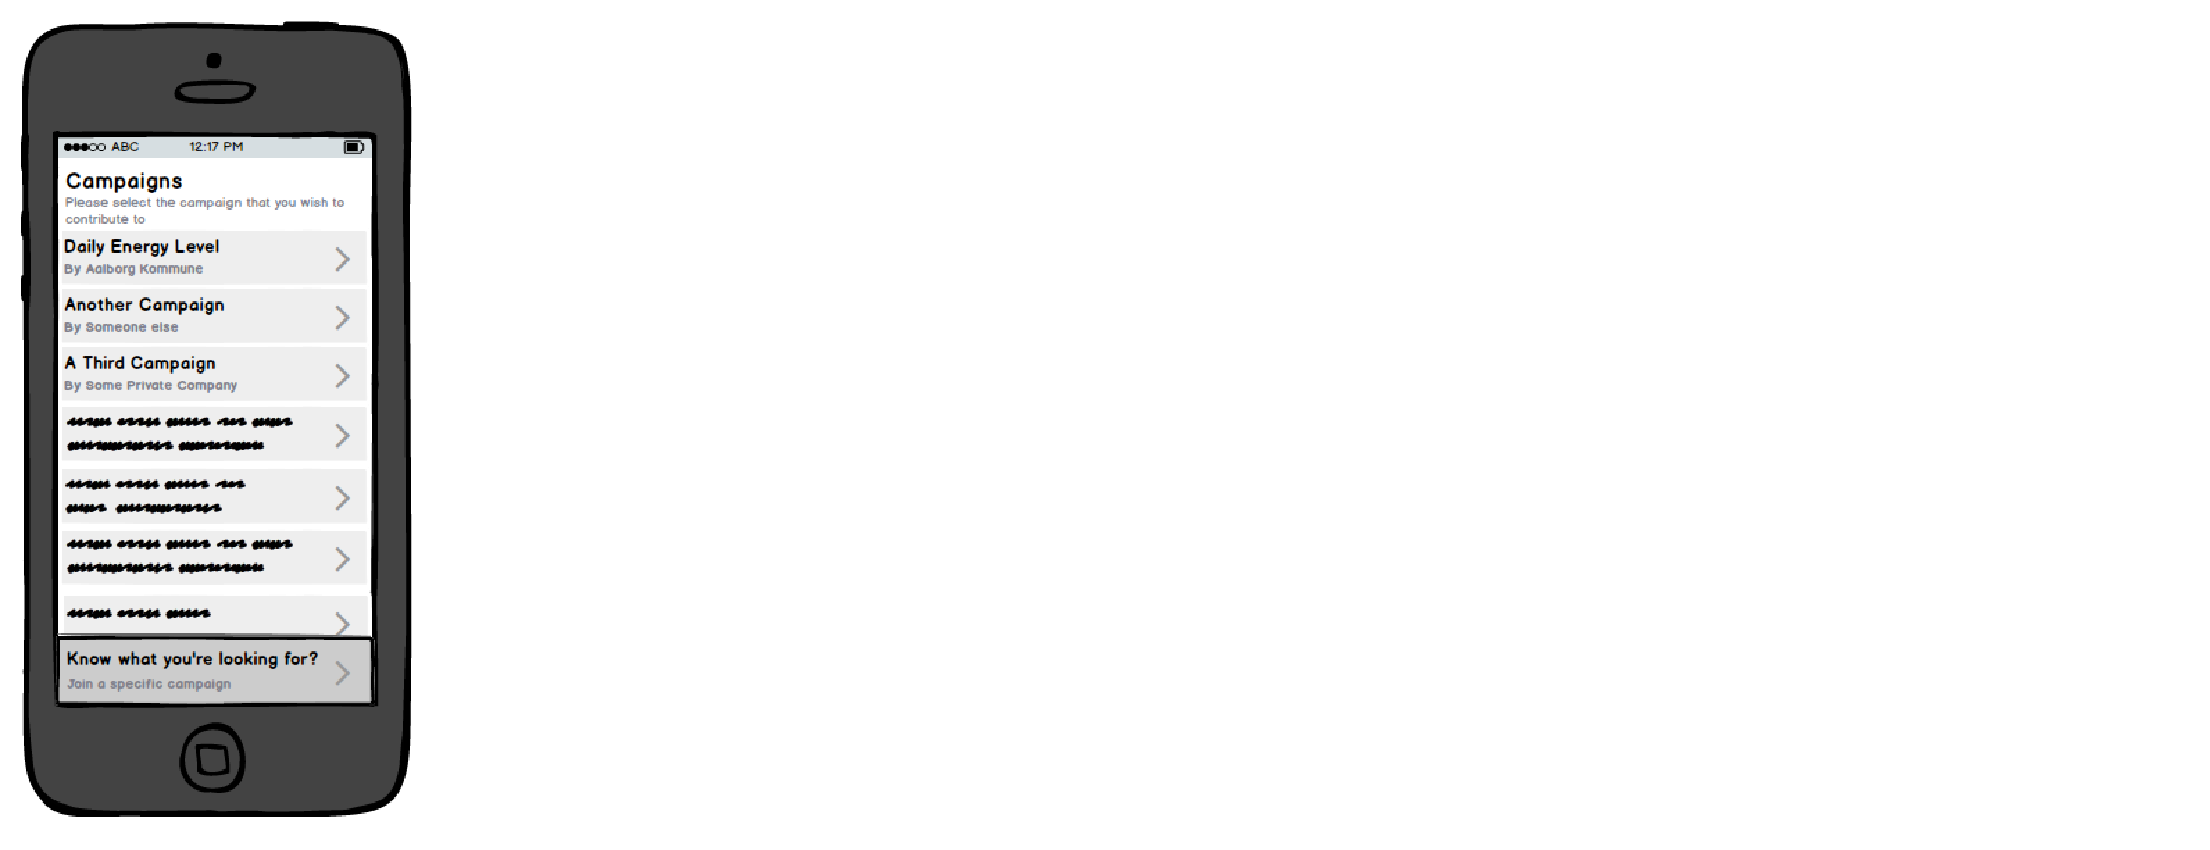
\includegraphics[width=.7\linewidth]{mockups/campaigns_list}
  \caption{Mockup.}
  \label{fig:mockup_public_campaigns}
\end{subfigure}%
\begin{subfigure}[!t]{.52\textwidth}
  \centering
  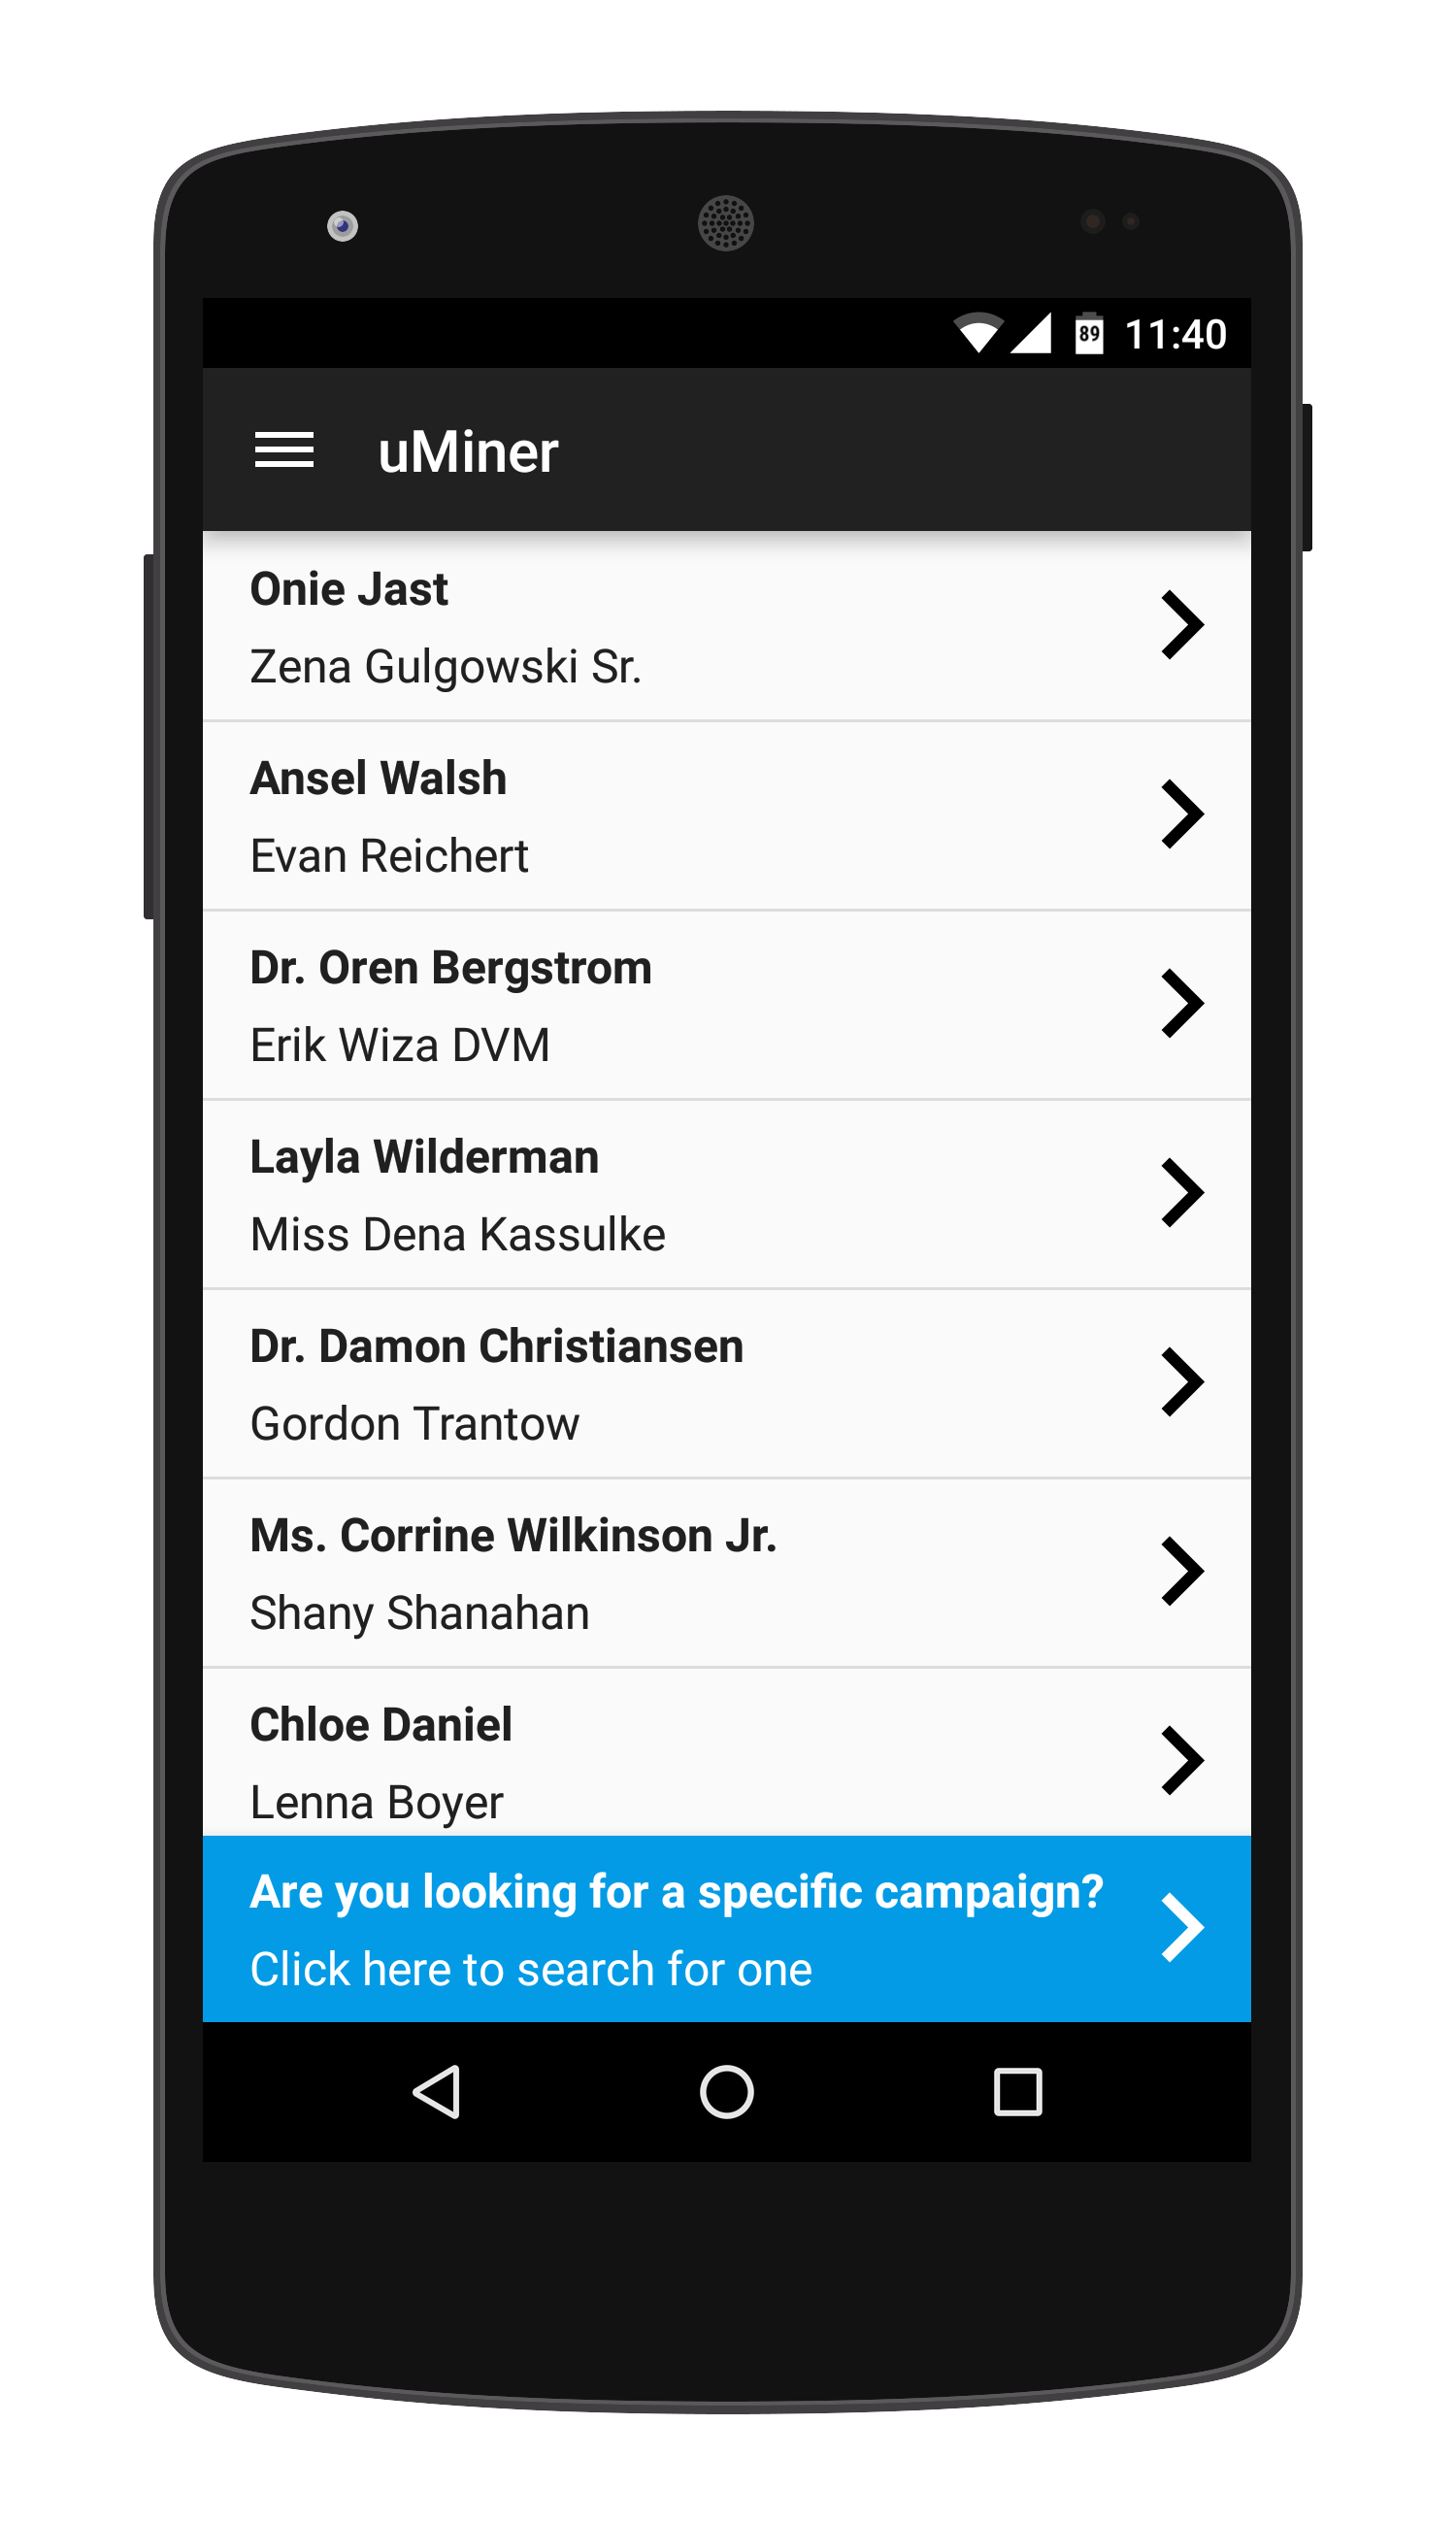
\includegraphics[width=.73\linewidth]{user_interfaces/client/client_public_campaigns_with_phone}
  \caption{Implementation.}
  \label{fig:implementation_public_campaigns}
\end{subfigure}
\caption{List of publicly available campaigns.}
\label{fig:public_campaigns}
\end{figure}
\FloatBarrier

An alternative way of finding campaigns, are through the view seen in \figref{fig:specific_campaign}. Here participants can enter a unique campaign identifier. If the identifier corresponds to a campaign, the participant will be redirected to a view similar to the one seen in \figref{fig:campaign_specification}. If not, he/she will be notified that the entered campaign identifier is invalid\todo{Dette afsnit skal ref til det sted hvor vi beskriver web-delen hvor man kan se hvilket ID campaignen har}. Throughout the project, we have thought of quite a number of different ways of allowing the participants to search for campaigns using different search criteria.

\begin{description}
 	\item[Quick Response Code (QR code)] could be utilized to give participants an easy way of subscribing to campaigns, simply by scanning a QR code. Customers would be able to distribute these QR codes through both digital and printed media. Furthermore, QR codes might be more easily relatable for participants, since they might be familiar with the concept from other domains.

 	\item[Specific search criteria] might help participants to find exactly what they want to contribute to. Participants might only want to contribute to campaigns with a scientific background, or campaigns that have next to no impact on battery life. Other criteria might be: limited amount of, or no questions in questionnaires; also some participants might not be willing to permit for specific sensors, so the possibility of searching for specific campaigns might be desirable.

 	\item[Prizes and other motivational factors] will potentially have a big impact on which campaigns gets contributed to. This means that the application could assist customers in getting more participants for their campaigns by displaying information regarding the prizes that customers might provide to willing participants. One could also imagine that participants could filter campaigns with or without prizes. 
\end{description} 


% Search for a campaign through a campaign identifier
\begin{figure}[!htbp]
\begin{subfigure}[!t]{.48\textwidth}
  \centering
  
\includegraphics[width=.7\linewidth]{mockups/join_specific_campaign}
  \caption{Mockup.}
  \label{fig:mockup_specific_campaign}
\end{subfigure}%
\begin{subfigure}[!t]{.52\textwidth}
  \centering
  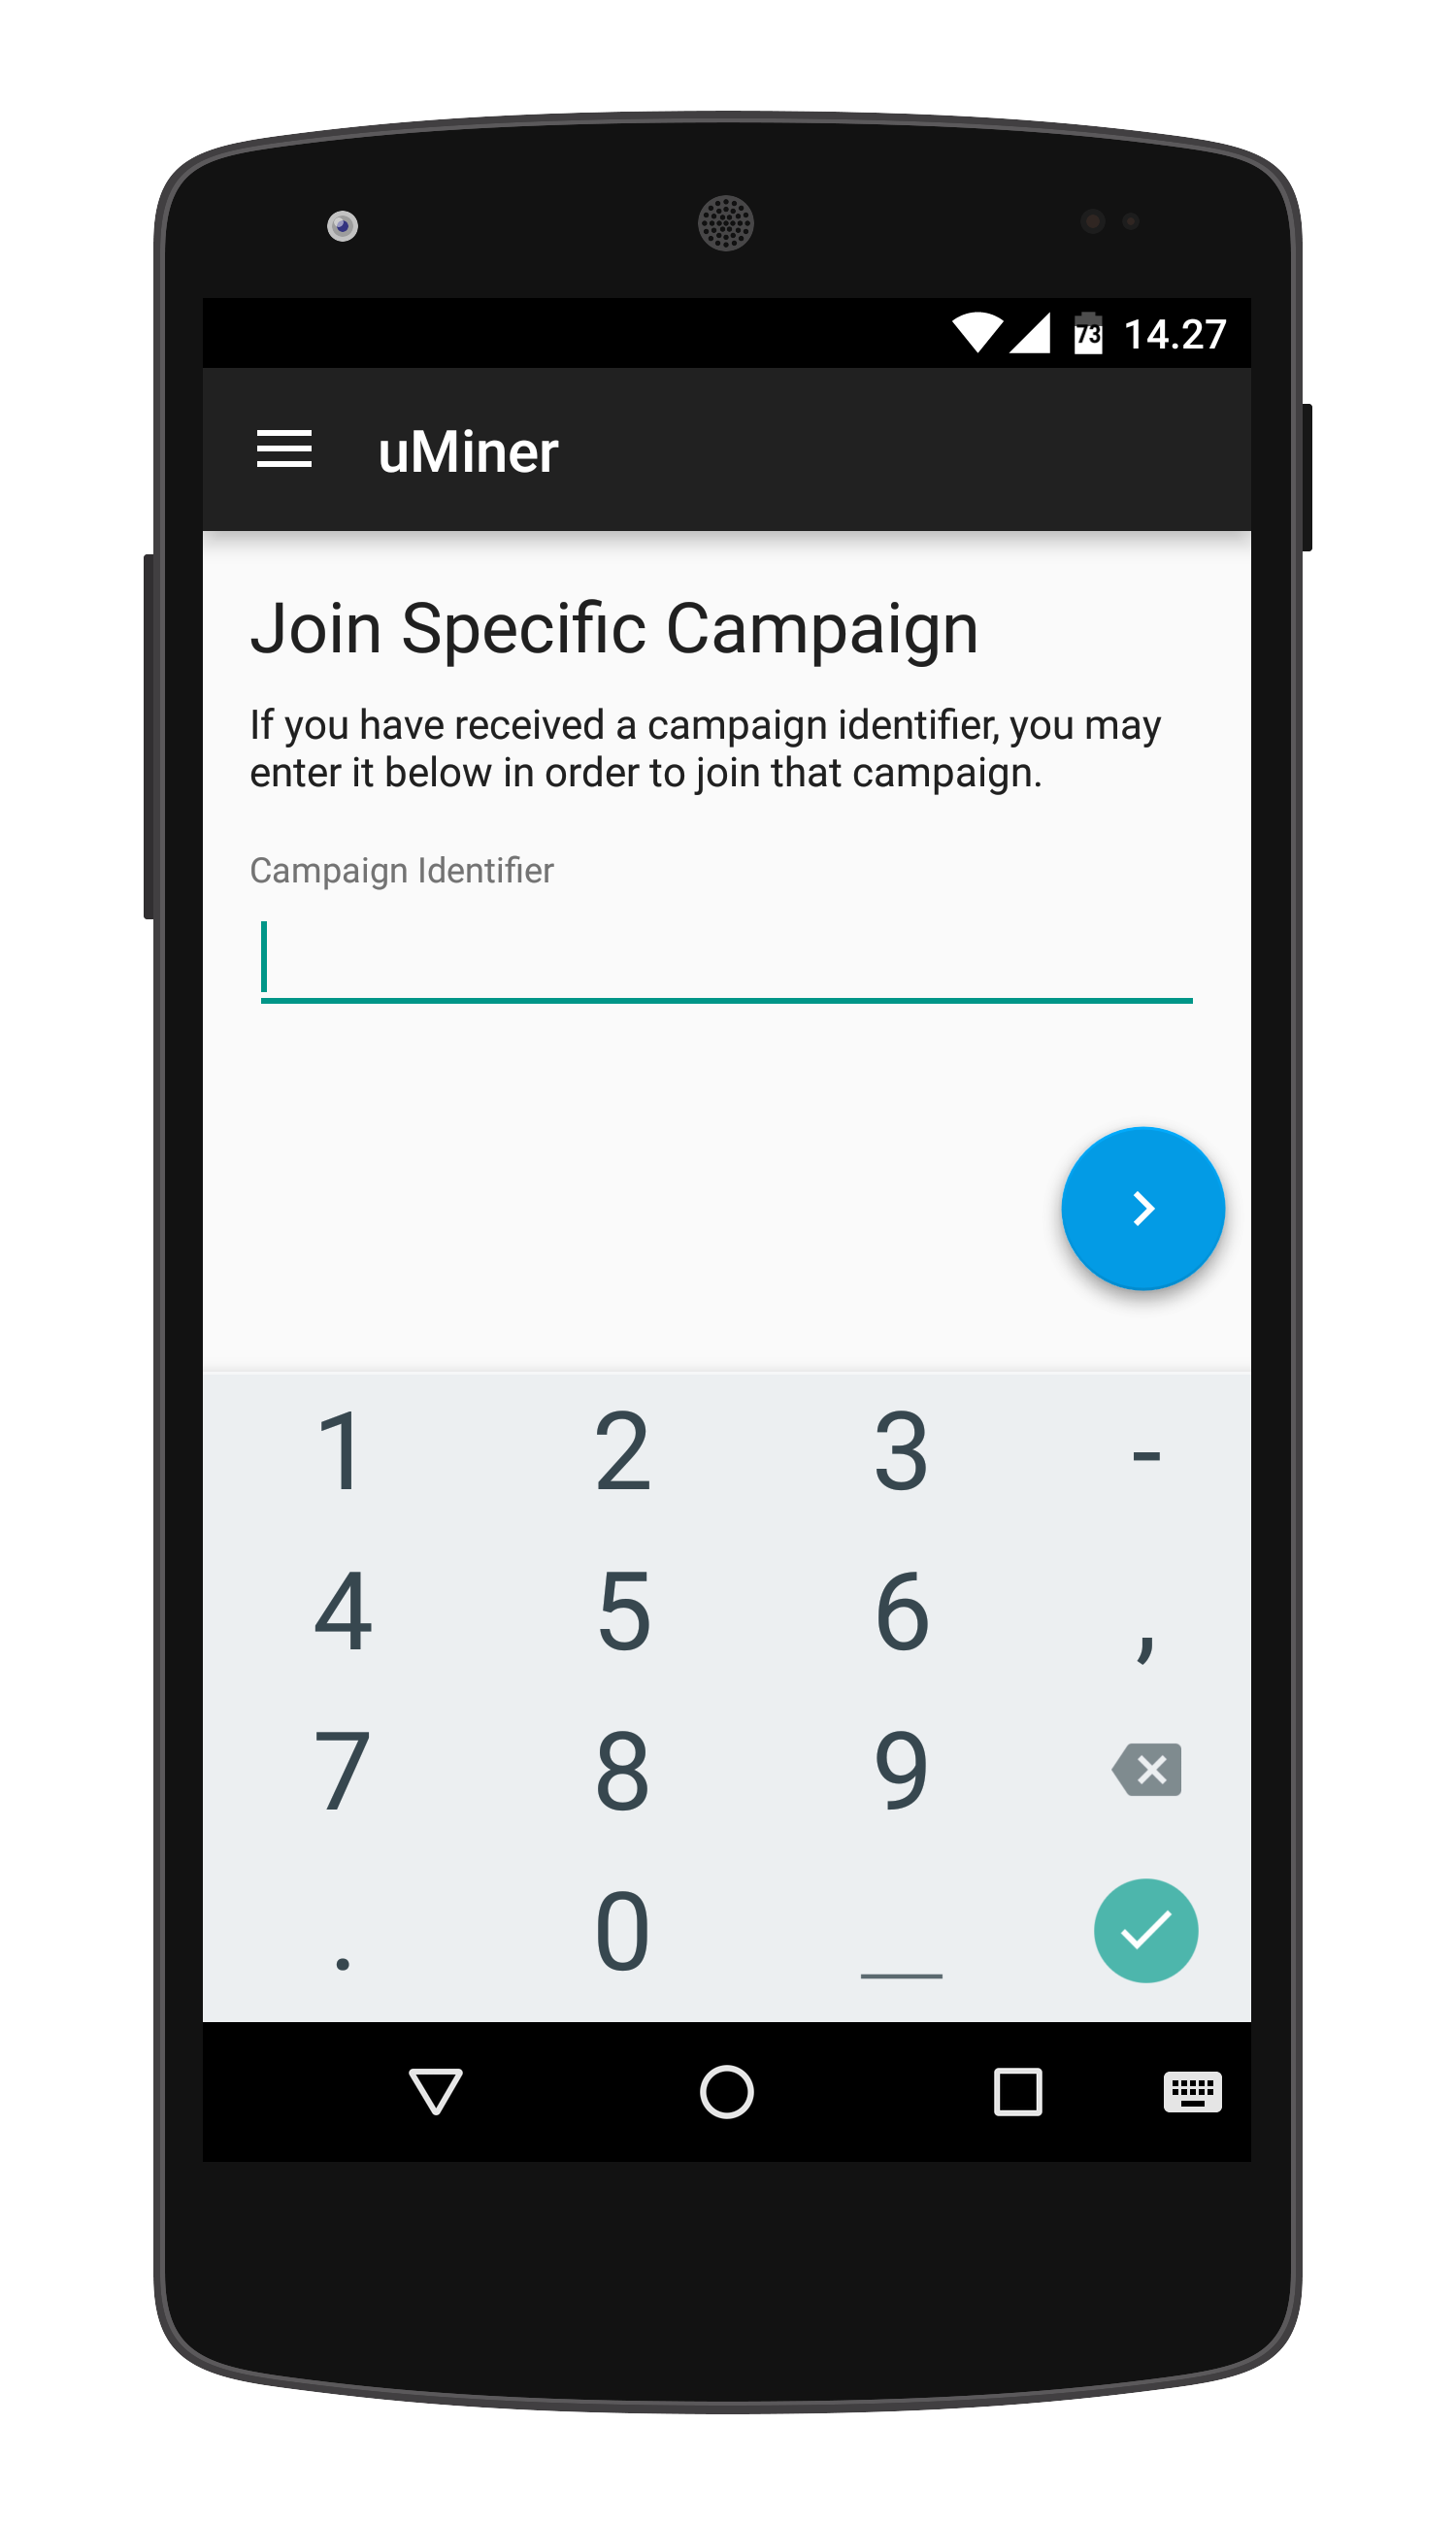
\includegraphics[width=.73\linewidth]{user_interfaces/client/client_join_specific_campaign_with_phone}
  \caption{Implementation.}
  \label{fig:implementation_specific_campaign}
\end{subfigure}
\caption{Search for a specific campaign using a campaign identifier.}
\label{fig:specific_campaign}
\end{figure}
\FloatBarrier

\subsection{Contributing to Campaigns}

To contribute to a specific campaign, participants must first find a campaign that the want to contribute to. This can be done through the campaign browser, previously shown in \figref{fig:public_campaigns} or by being introduced to a campaign externally. The participants must then navigate a campaign specification view, similar to the one seen in \figref{fig:campaign_specification}. Here, participants can view the details of the campaign; after reviewing this information, they can then decide if they want to contribute by subscribing to the campaign, which will be done by pressing the green button.
\\\\
If for any reason, participants no longer wishes to contribute to the campaign that they subscribed to, they can find the specification for this campaign. When viewing the campaign that they have subscribed to, the green subscribe button will instead be a red unsubscribe button, as seen in \figref{fig:leave_campaign_no_dialog}. Pressing this button, will trigger a confirmation dialog, as seen in \figref{fig:leave_campaign_dialog}. If the participants confirms this, by pressing yes, all data collection will immediately stop, however, participants may still be asked questions, depending on the campaign.

\todo[inline]{Overvej om vi skal snakke om participatory design her? Folk vælger jo selv om de vil være med, og hvad de gerne vil bidrade til}

\todo[inline]{Reference til hvordan vi indsamler data i baggrunden}

% Campaign specification
\begin{figure}[!htbp]
\begin{subfigure}[!t]{.48\textwidth}
  \centering
  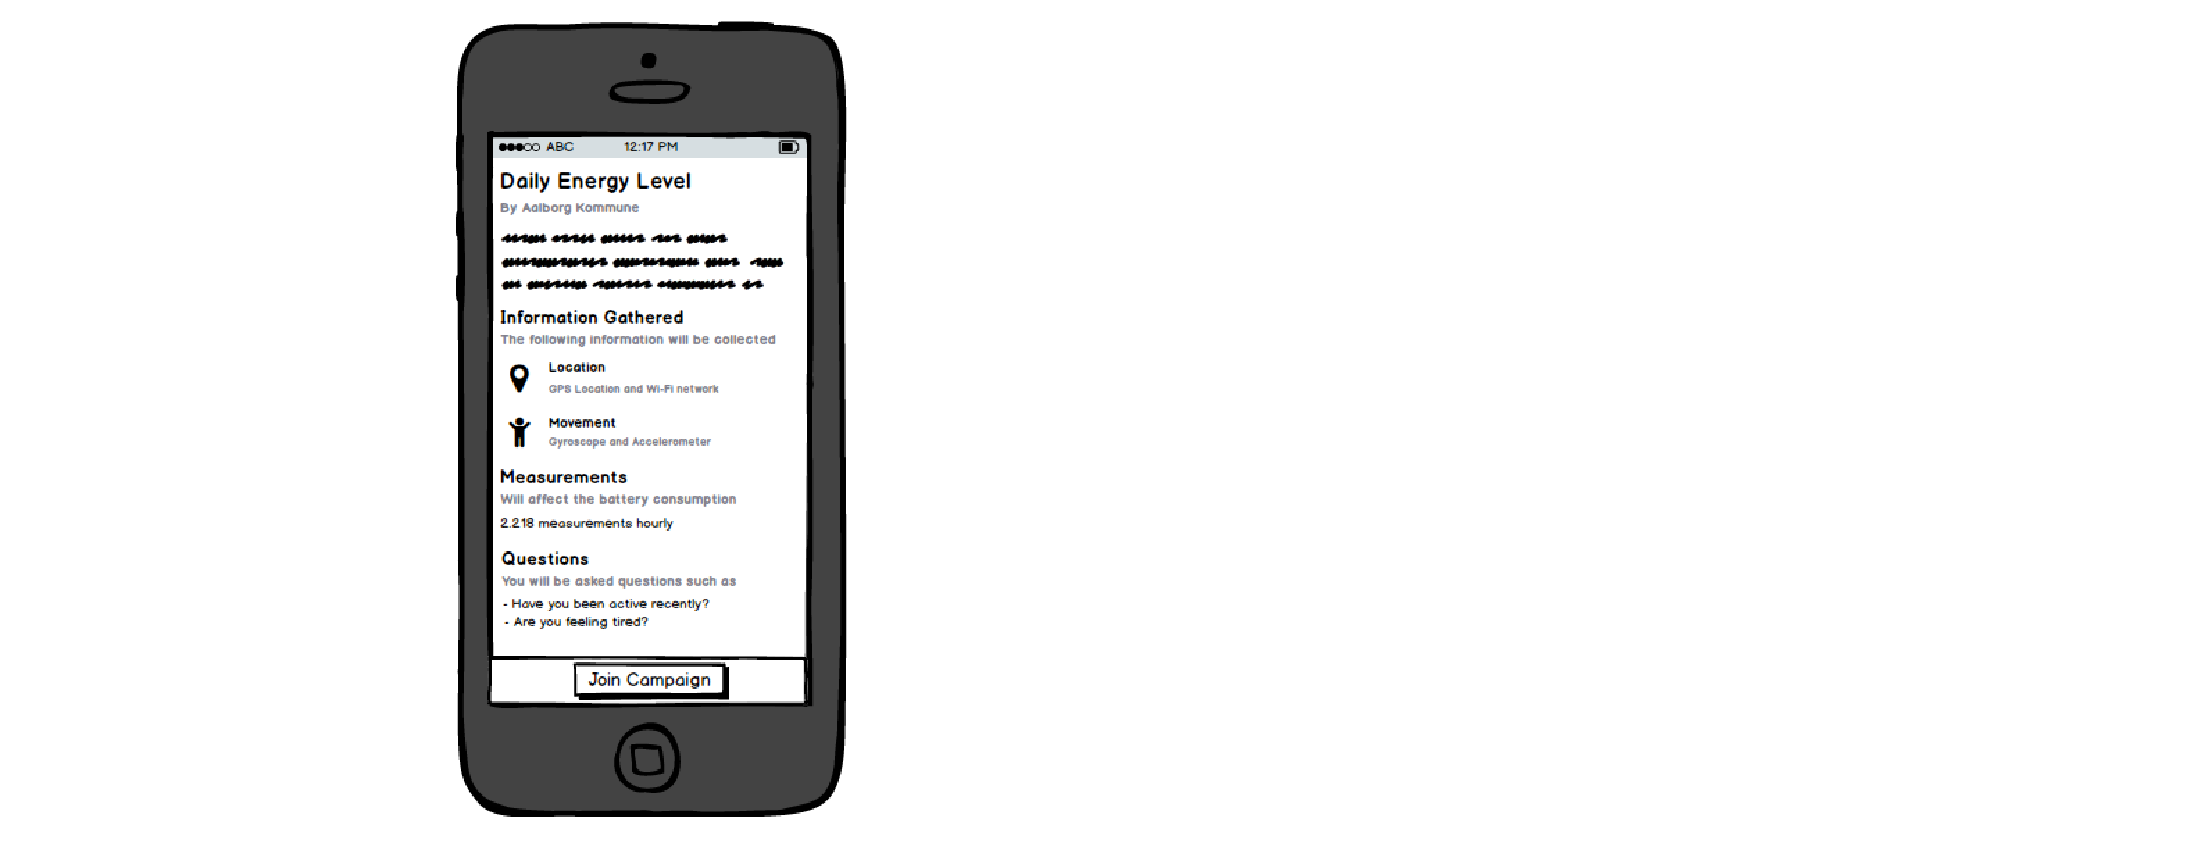
\includegraphics[width=.7\linewidth]{mockups/campaign_specification}
  \caption{Mockup.}
  \label{fig:mockup_campaign_specification}
\end{subfigure}%
\begin{subfigure}[!t]{.52\textwidth}
  \centering
  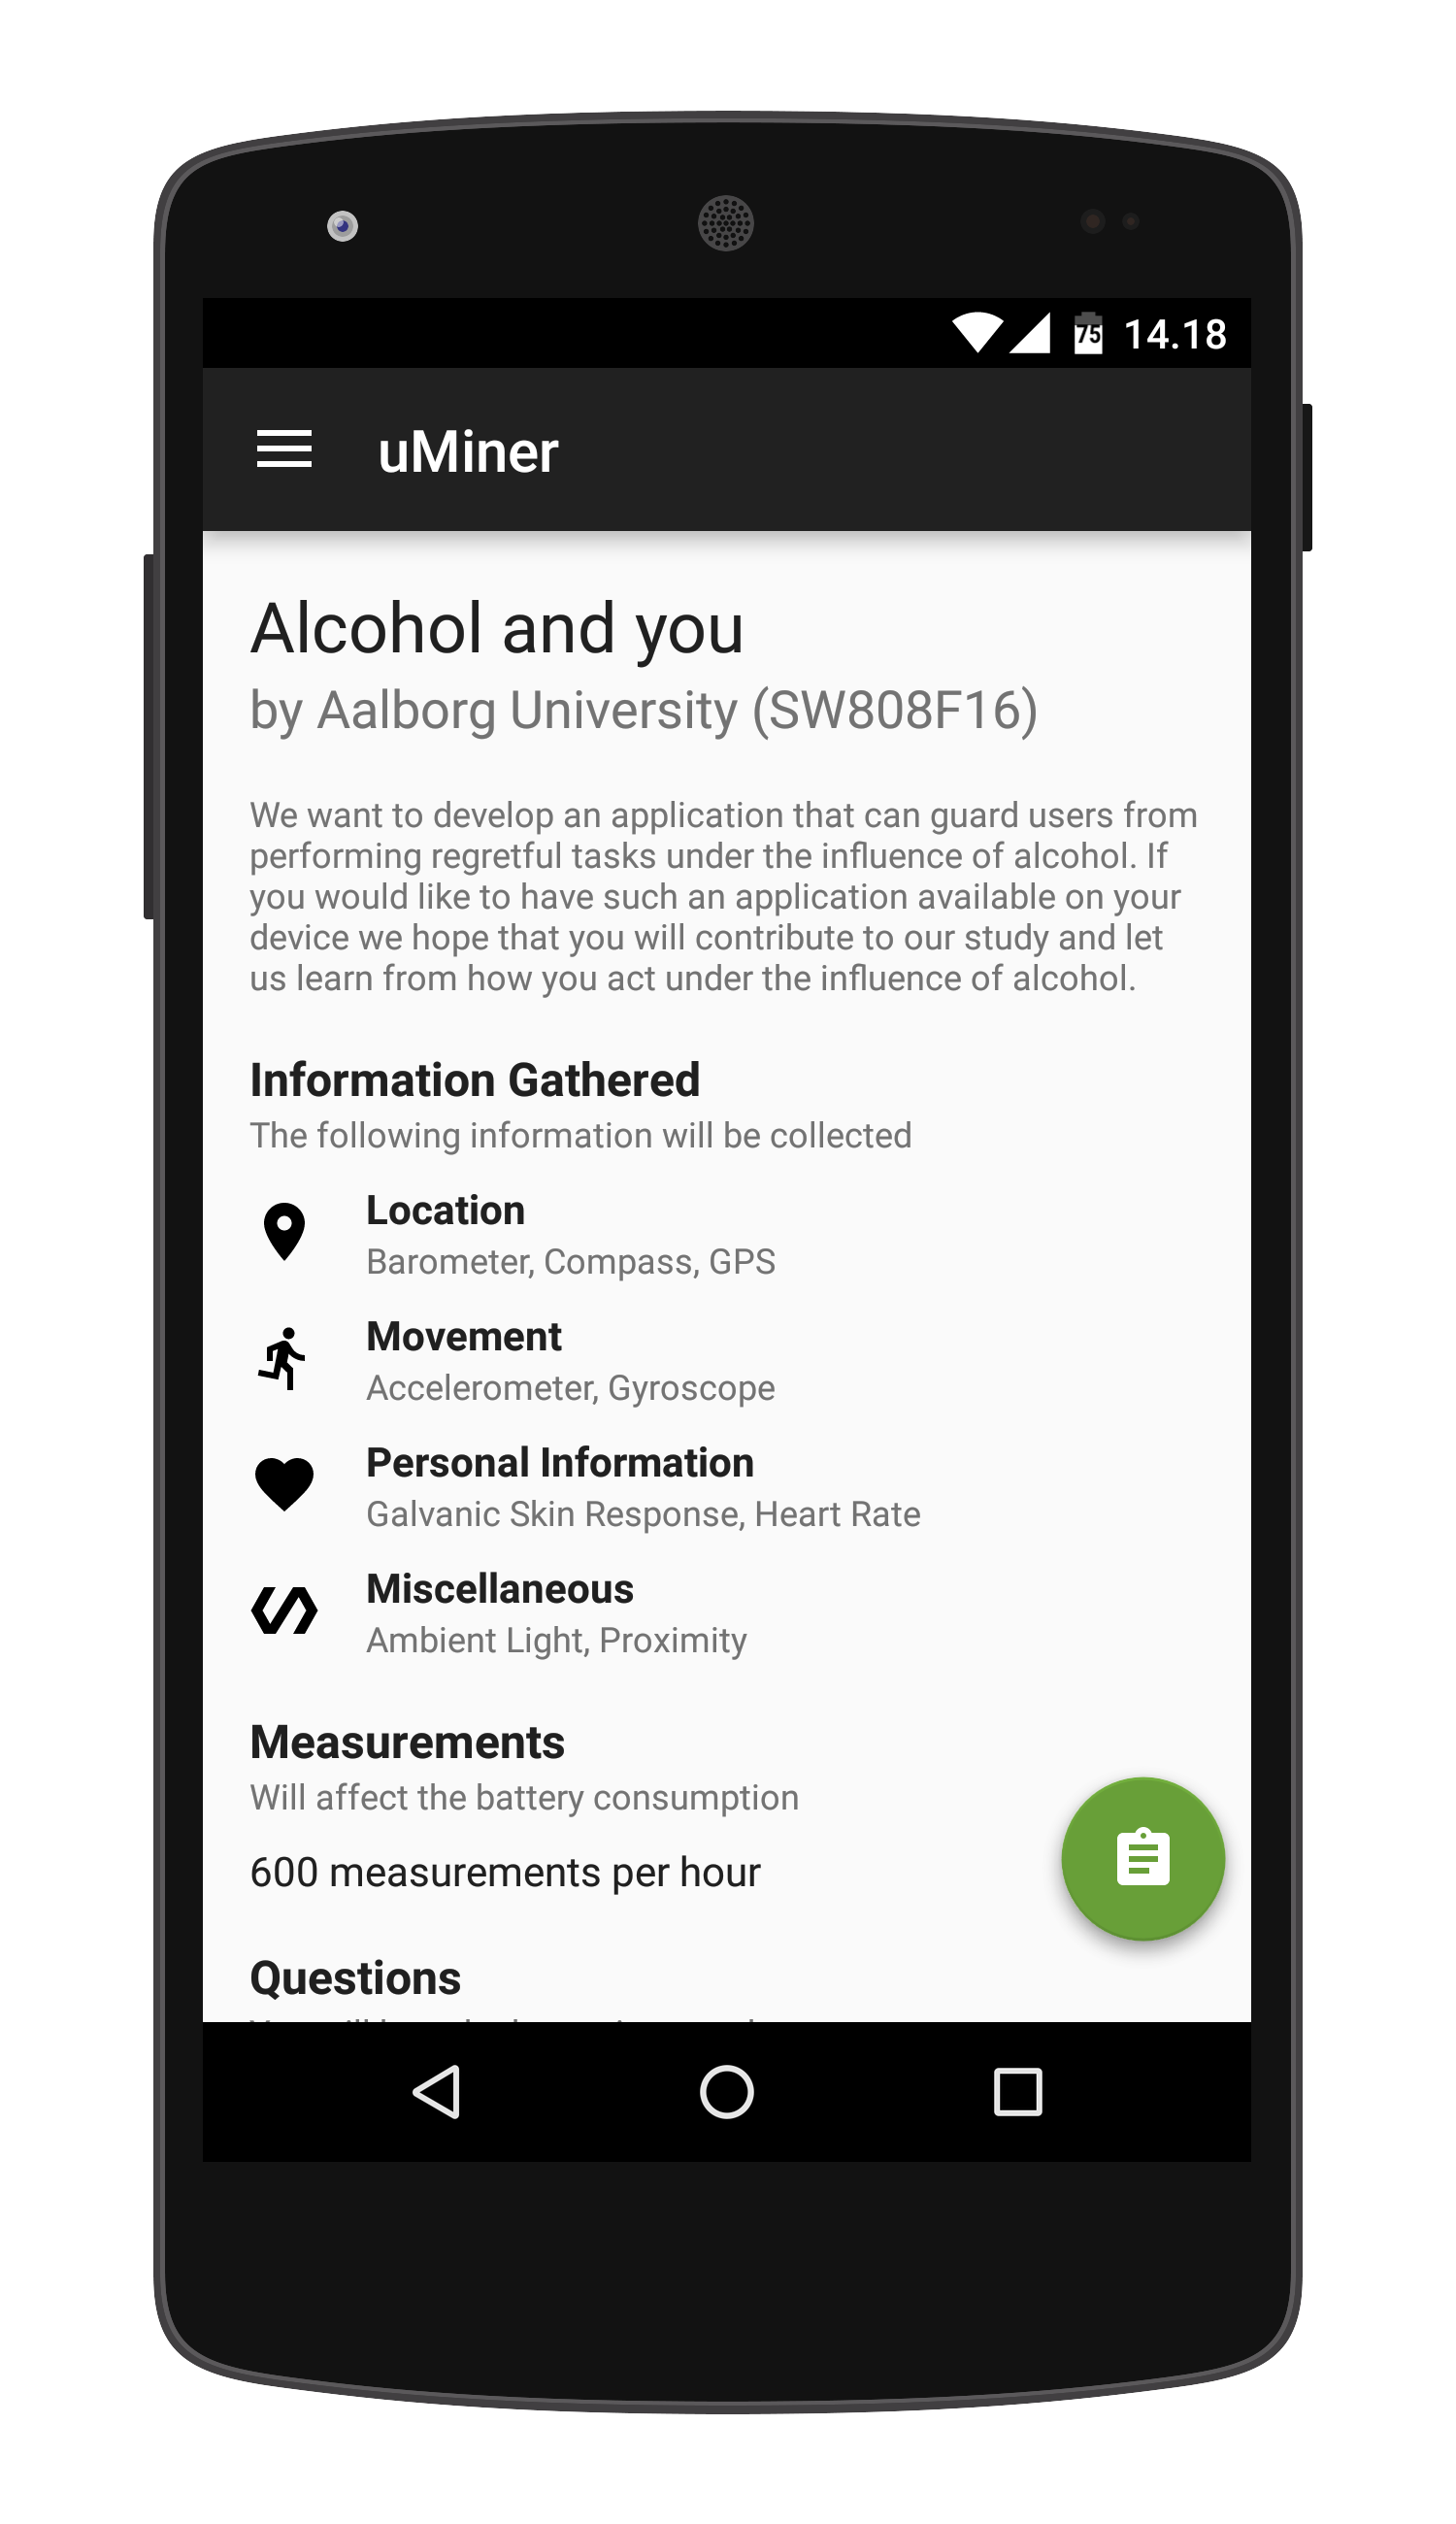
\includegraphics[width=.73\linewidth]{user_interfaces/client/client_campaign_specification2_with_phone}
  \caption{Implementation.}
  \label{fig:implementation_campaign_specification}
\end{subfigure}
\caption{Campaign specification view.}
\label{fig:campaign_specification}
\end{figure}
\FloatBarrier

% Leave campaign and dialog
\begin{figure}[!htbp]
\begin{subfigure}[!t]{.50\textwidth}
  \centering
  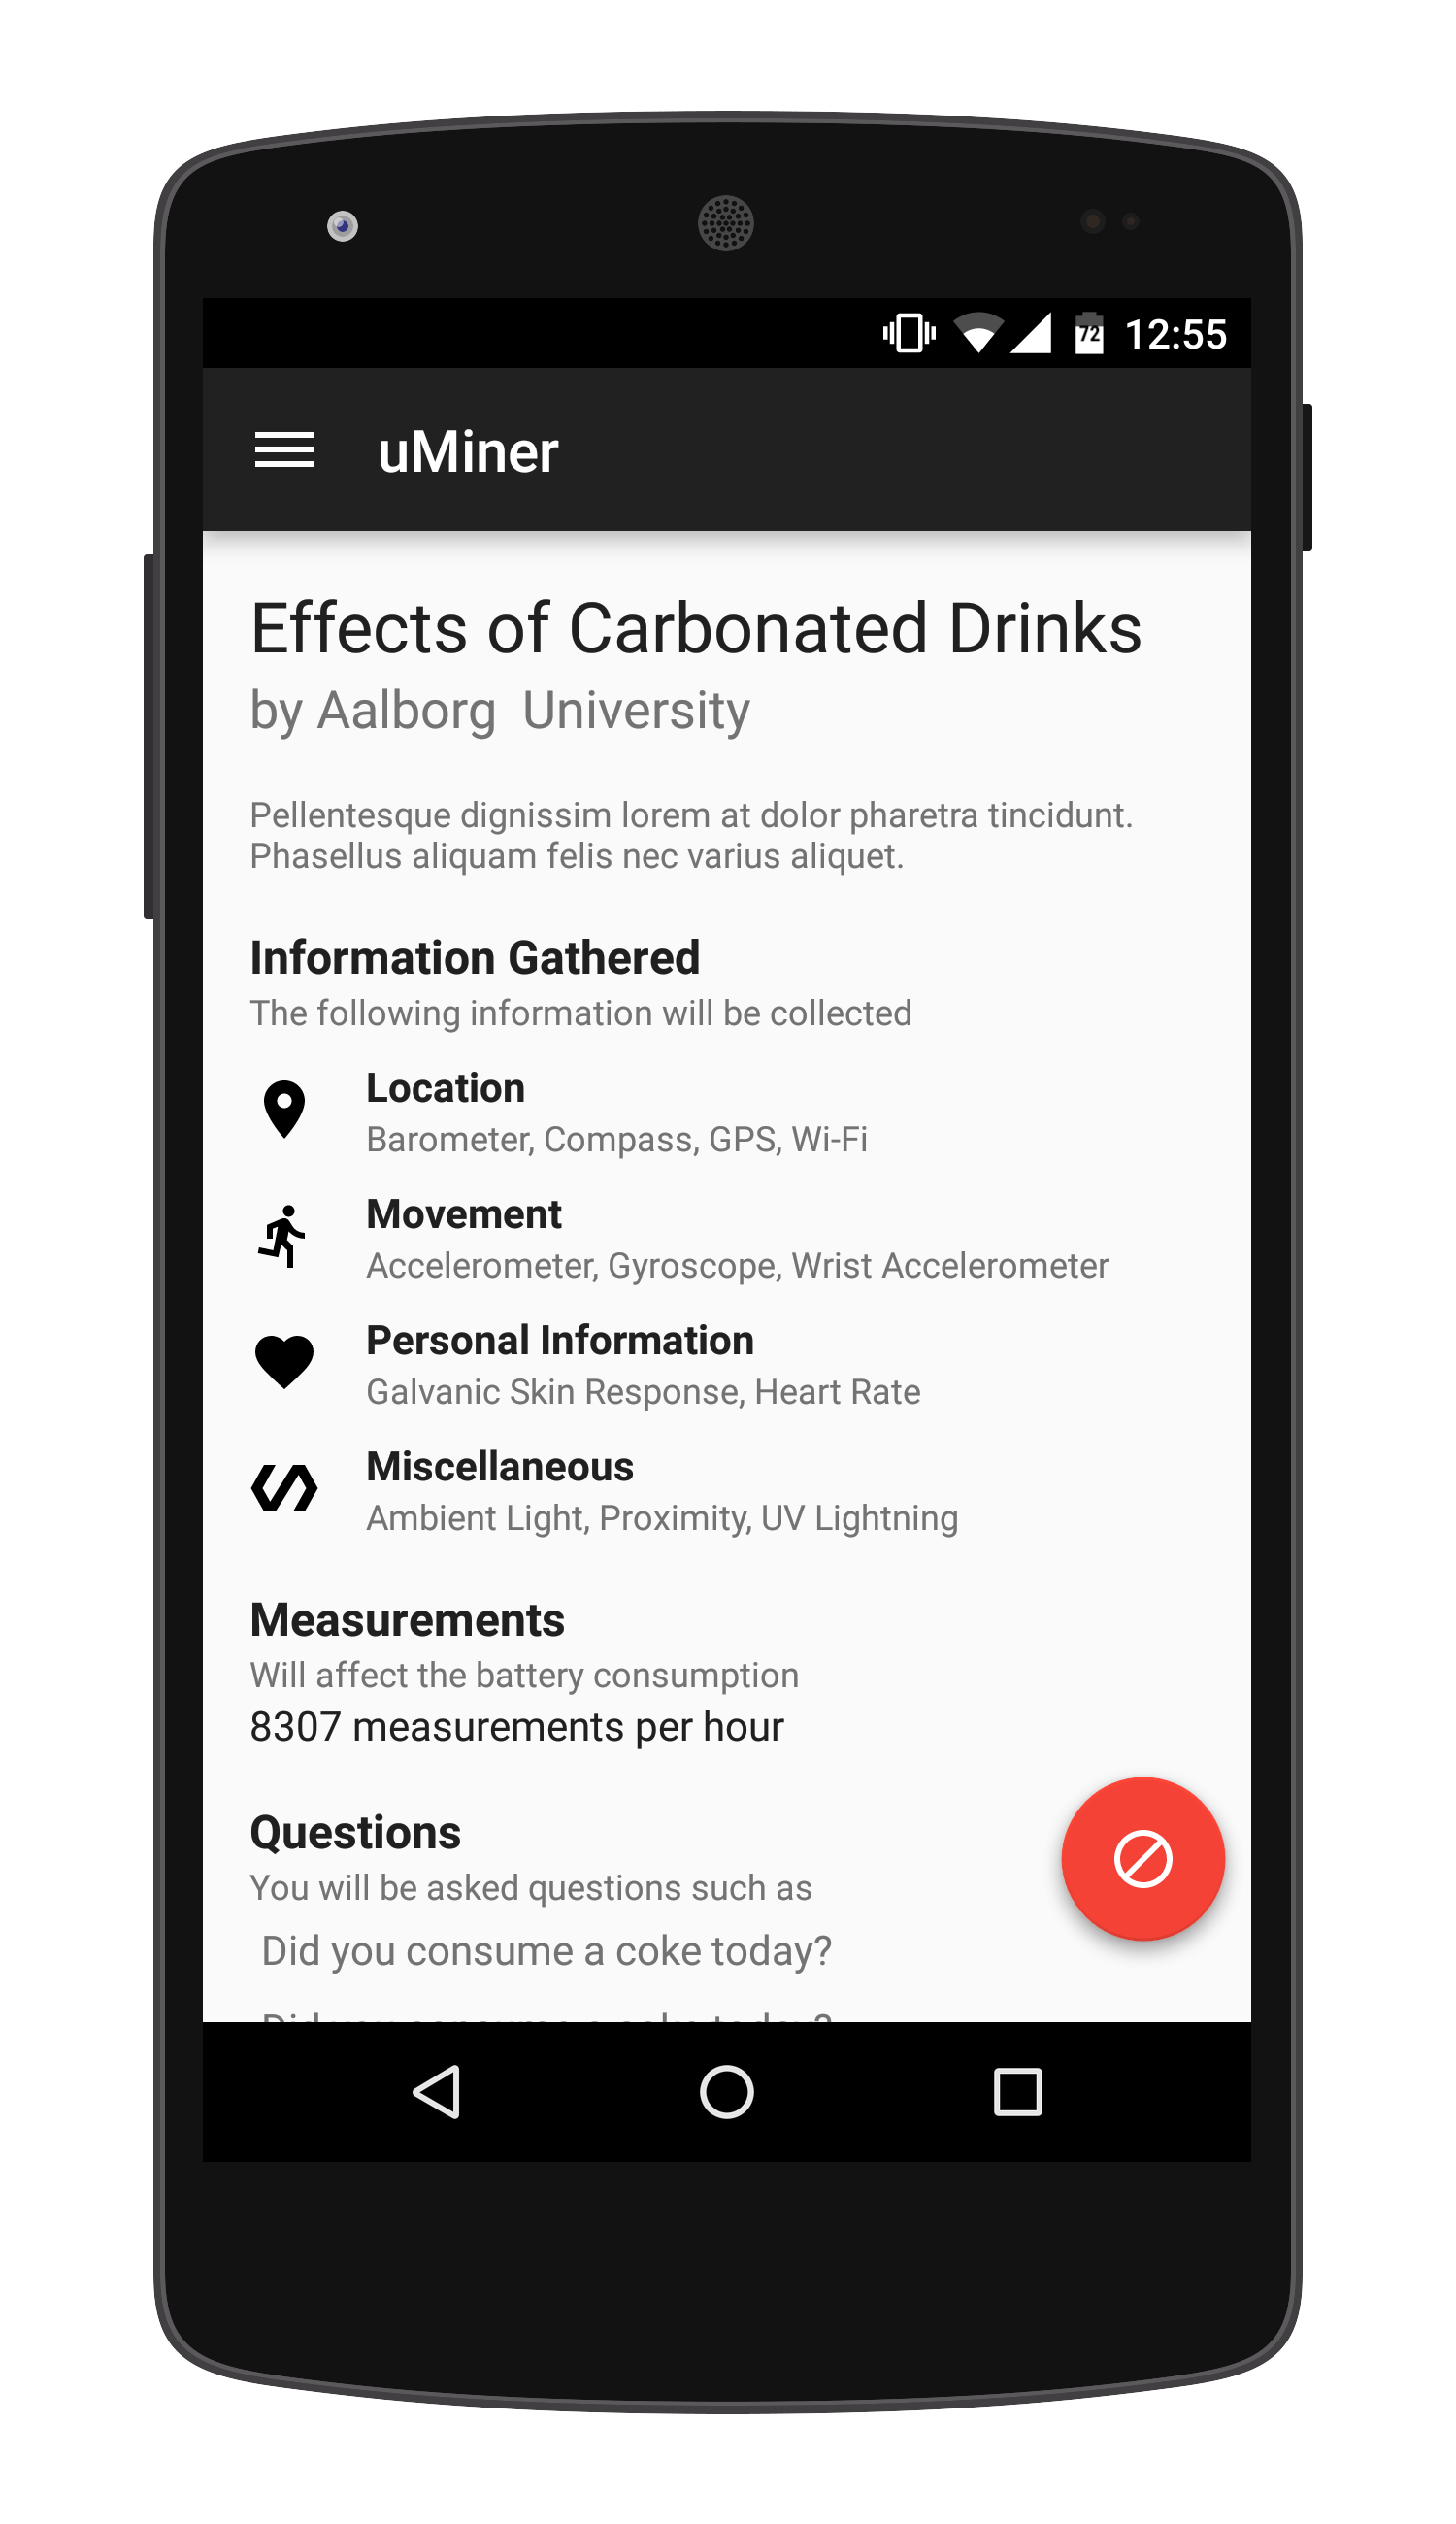
\includegraphics[width=.73\linewidth]{user_interfaces/client/client_leave_campaign_no_dialog_with_phone}
  \caption{Specification with leave button.}
  \label{fig:leave_campaign_no_dialog}
\end{subfigure}%
\begin{subfigure}[!t]{.50\textwidth}
  \centering
  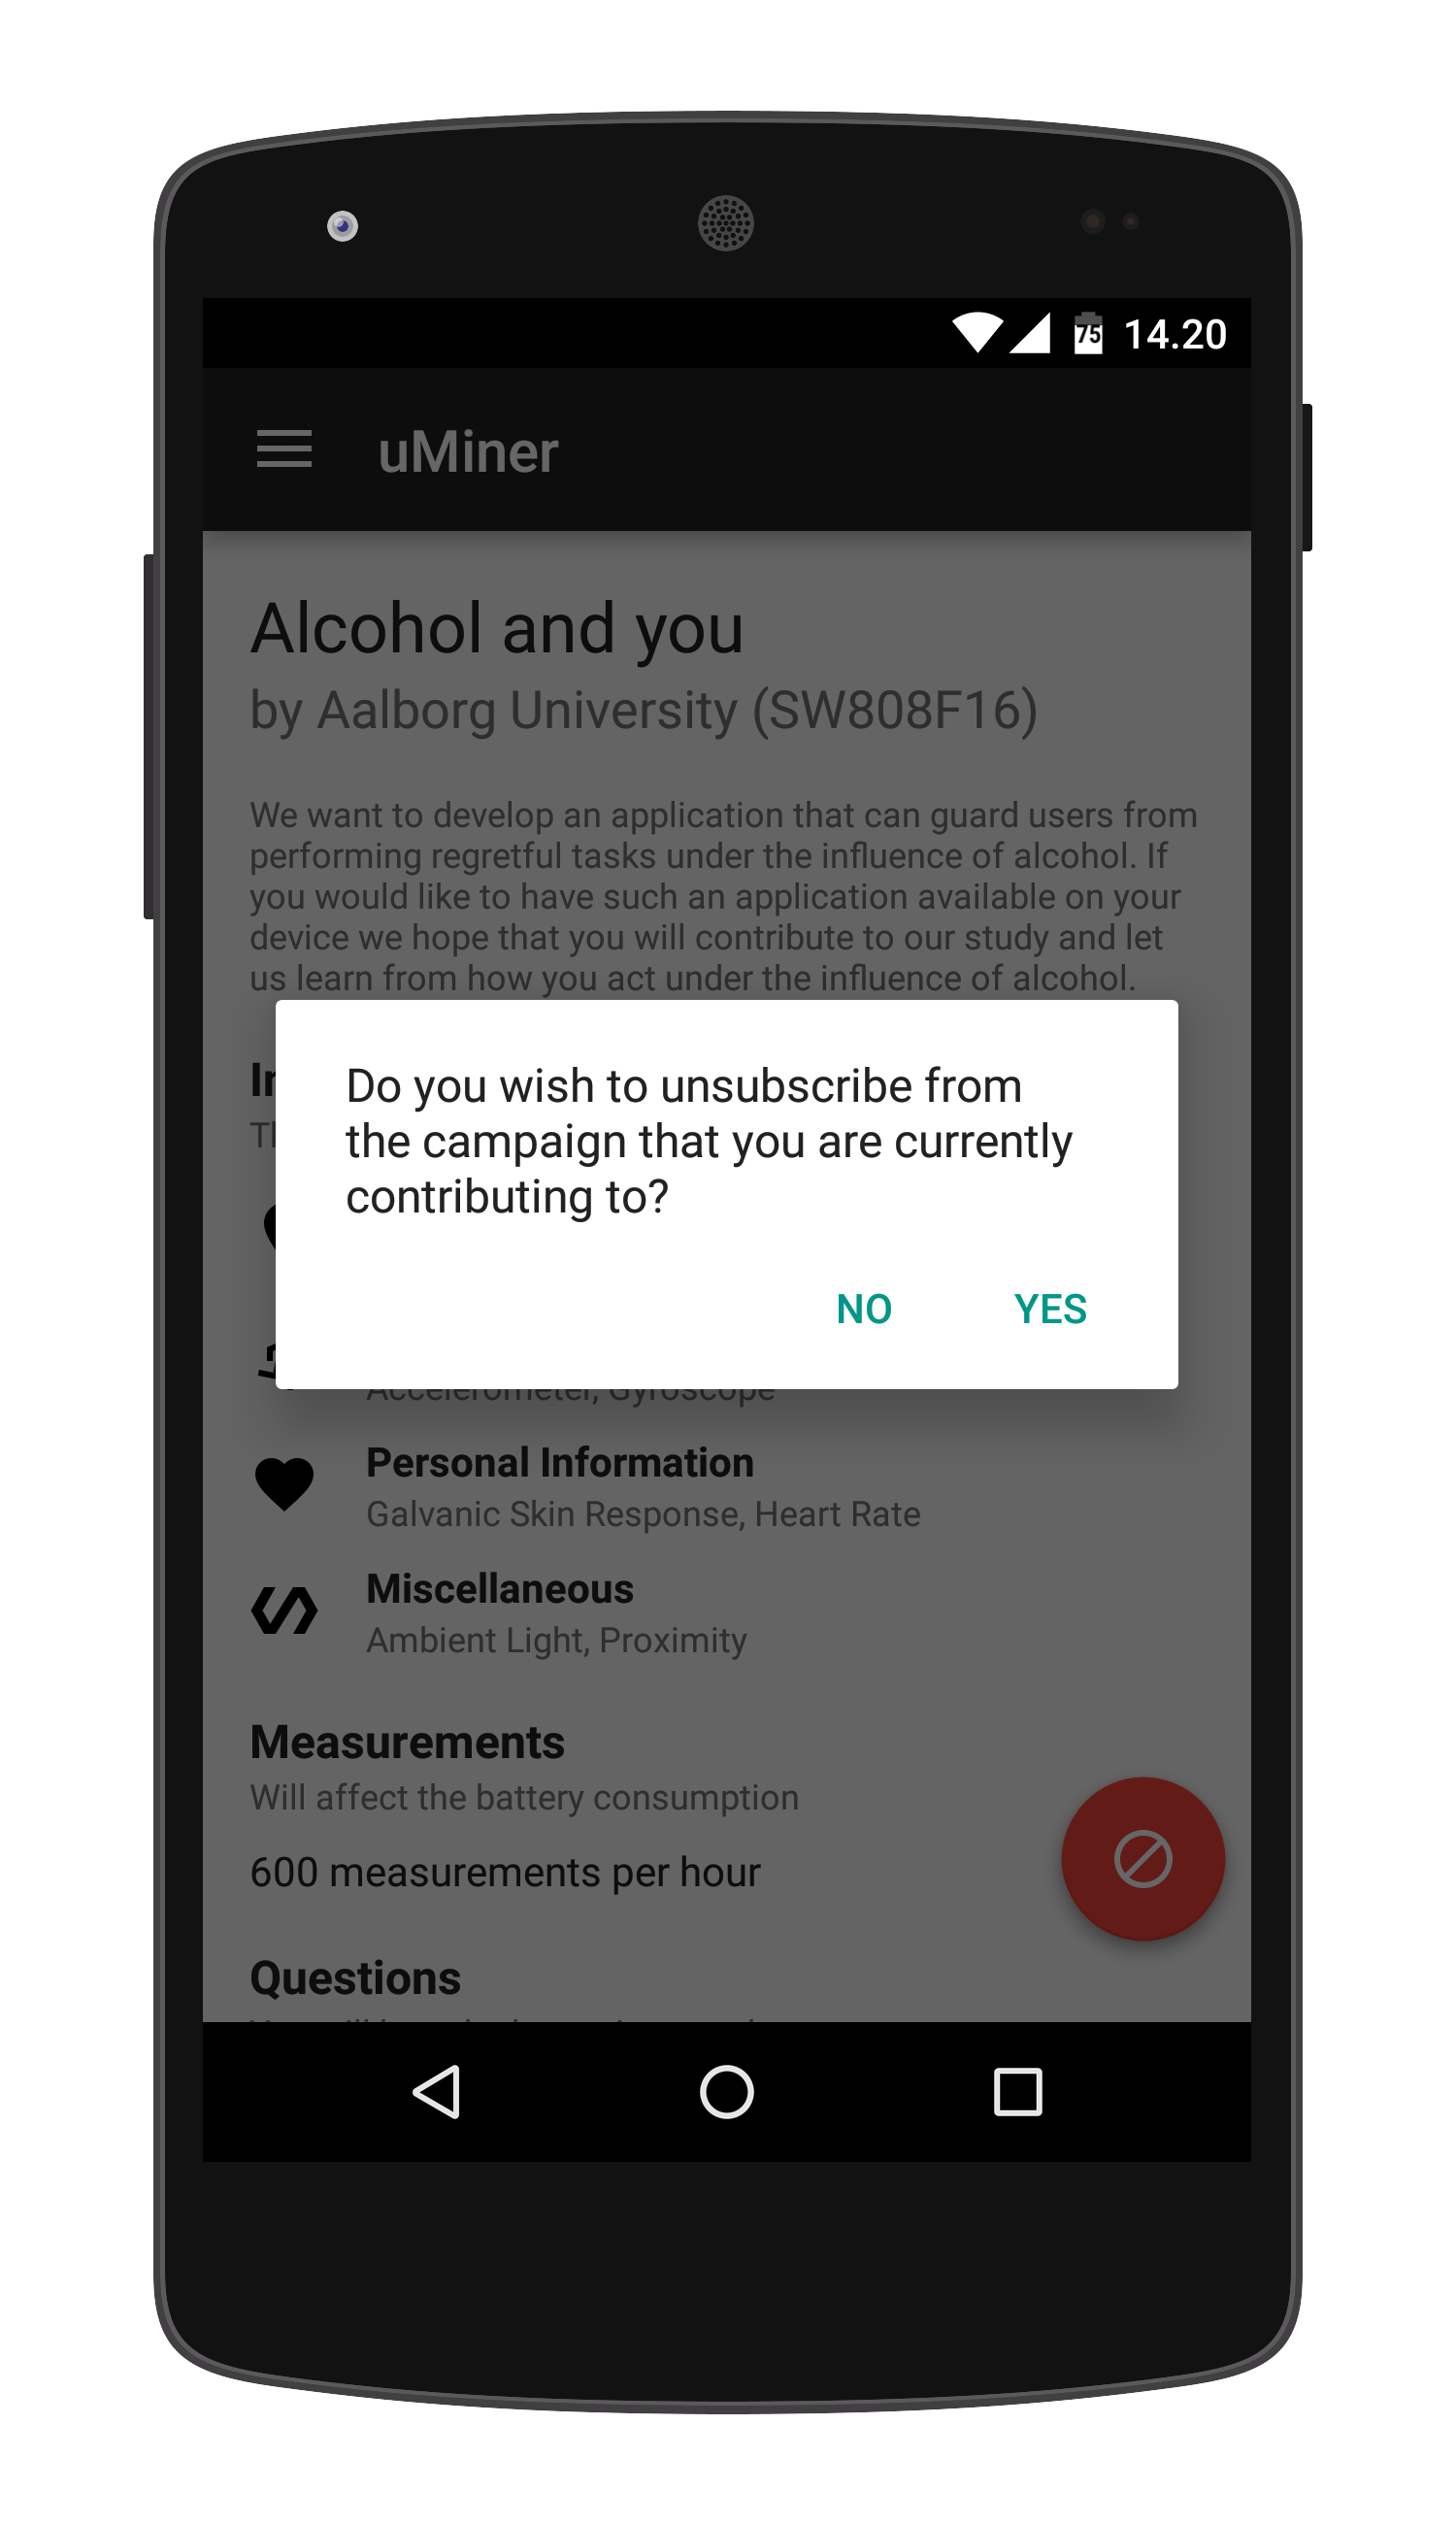
\includegraphics[width=.73\linewidth]{user_interfaces/client/client_leave_campaign_with_phone}
  \caption{Confirmation dialog.}
  \label{fig:leave_campaign_dialog}
\end{subfigure}
\caption{Leaving a campaign.}
\label{fig:leave_campaign}
\end{figure}
\FloatBarrier

\subsection{Answering Questionnaires}
\label{sub:answering_questionnaired}

Some campaigns might request that the participants answers a questionnaire once in a while. This might happen when the participant has closed the application, or when the participant is not even using the phone. To accompany this, we chose to use notifications to inform the participant when they should answer questionnaires, which can be seen in \figref{fig:answering_questionnaire_notification}. When the notification is pressed, the application is opened with a specific activity, which can be seen in \figref{fig:answering_questionnaire_answering}. In the current system, customers can only specify yes/no questions, but we have thought of different concepts for labeling the collected information.

\begin{description}
  	\item[Complex questions] might be required for customers to get a better understanding of the label. Currently, only yes/no questions can be included in a questionnaire, however, customers might be interested asking more complex questions, such as: \emph{Which of the following statements would describe your current situation best?} or \emph{Please provide a small description of your current mood}. Questions such as the latter might be harder for customers to interpret, but techniques such as  sentiment analysis could be applied here. Ideally, the system should not limit the customer in defining what label they would like to retrieve, i.e. customers should be able to define whatever kind of question, or activity, they wish for participants to perform \todo{Her vil jeg gerne beskrive at der er mange metoder som kunderne kan bruge for at få information omkring dataen - så vi skal ikke spænde ben for dem på nogen som helst måde. Måske skal vi evt. overveje om vi skal skrive at de selv kan skrive activities?}. 

  	\item[Answer dependent questions] might be desired by customers to get a more detailed label, e.g. if the participants answers \emph{yes} to $q_1$, ask him $q_2$, otherwise ask $q_3$. Defining questions depending on the outcome of previous questions could become a complex task, and the customers might need some aid to visualize the questionnaire. Decision diagrams could be useful for this \todo{Er det nødvendigt med et eksempel her?}.
\end{description}

In the current application, questionnaires are triggered, and showed to the user, either in the start or the end of a snapshot \todo{insæt reference}. This will cause the time of questionnaires to be relative to the time that the participants subscribed to the campaign. This might complicate things when trying to build a machine intelligence based model around the collected data, because the label, and time of data collection is skewed between contributers. Because of this, alternative triggers could be desired by customers; some of our considerations are described below.

\begin{description}
   	\item[Timely fixed triggers] might be useful to ensure that all participants are notified regarding questionnaires simultaneously, i.e. at a specific time of day. This might cause gathered information to be more easily related. Furthermore, customers might be interested in asking participants regarding something, only at a specific time, e.g. in the morning (after finishing sleeping). 

   	\item[Event triggers] could be useful since participants is answering questions based on their own memory. So instead of waiting a fixed amount of time, triggers could be event based. This would prompt participants to answer questionnaires when a specific even occurs, e.g. when returning home, finished a call, etc.    
\end{description}    

% Answering questionnaires
\begin{figure}[!htbp]
\begin{subfigure}[!t]{.50\textwidth}
  \centering
  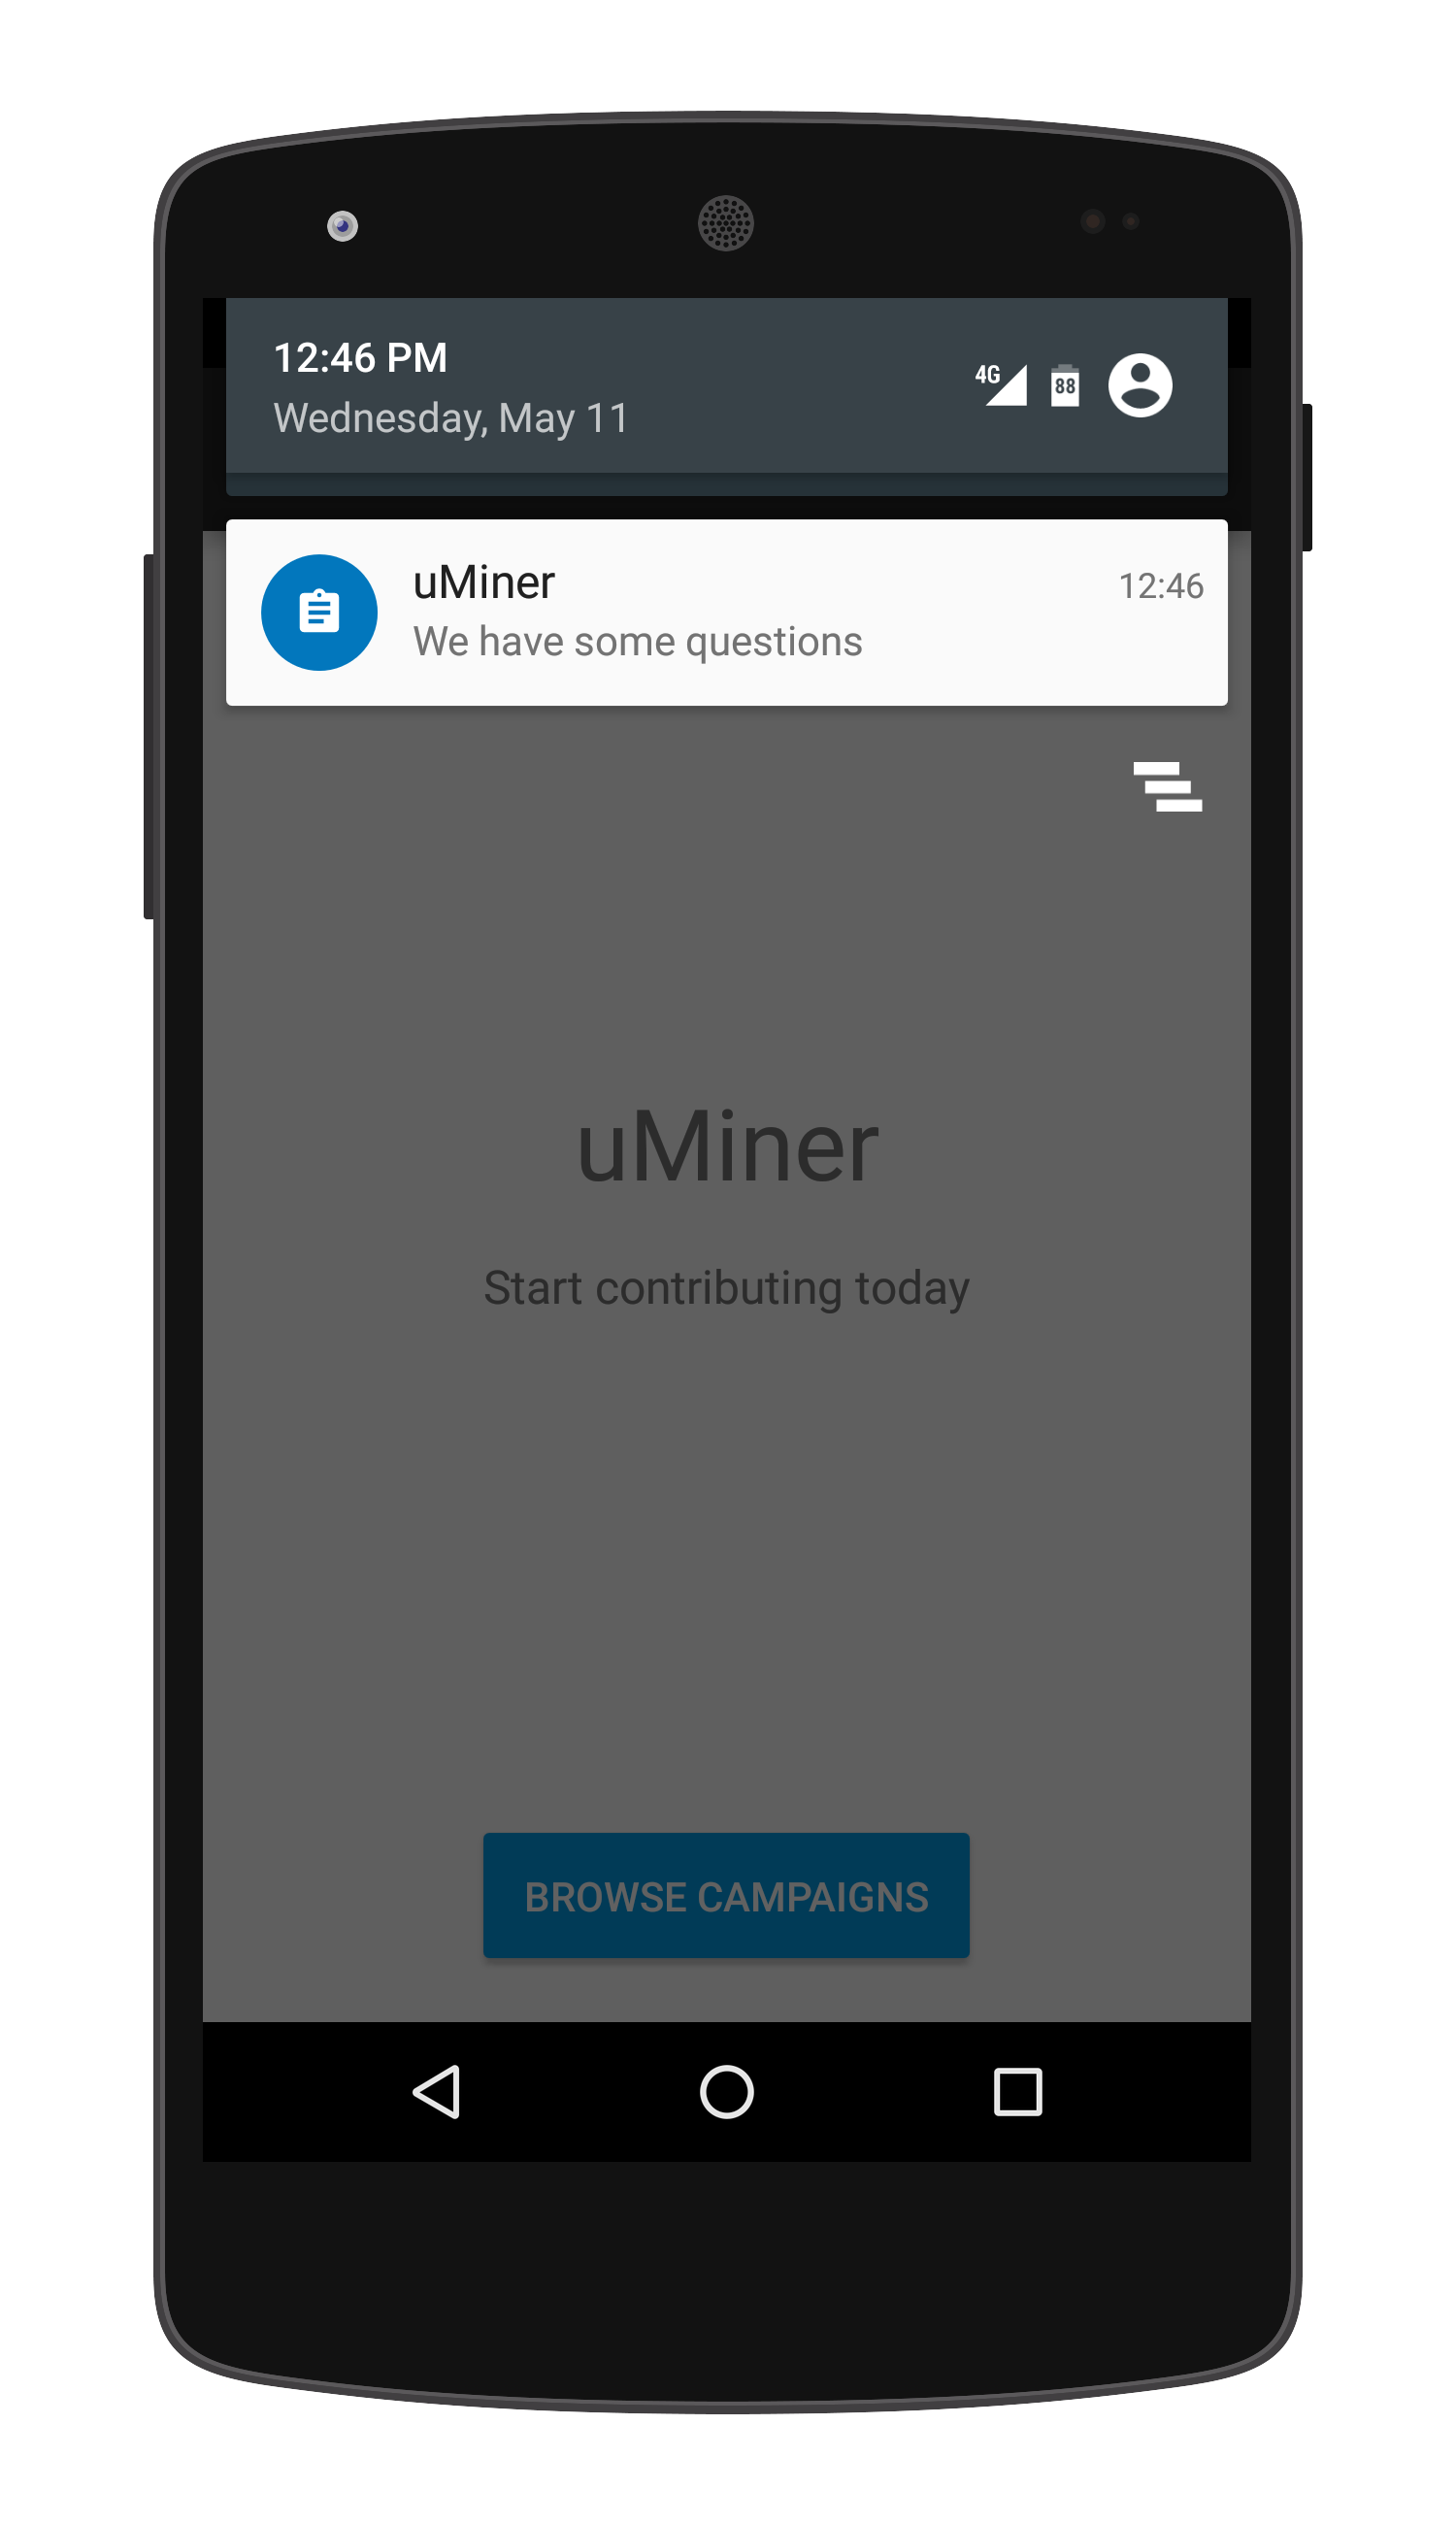
\includegraphics[width=.73\linewidth]{user_interfaces/client/client_notification_with_phone}
  \caption{Questionnaire notification.}
  \label{fig:answering_questionnaire_notification}
\end{subfigure}%
\begin{subfigure}[!t]{.50\textwidth}
  \centering
  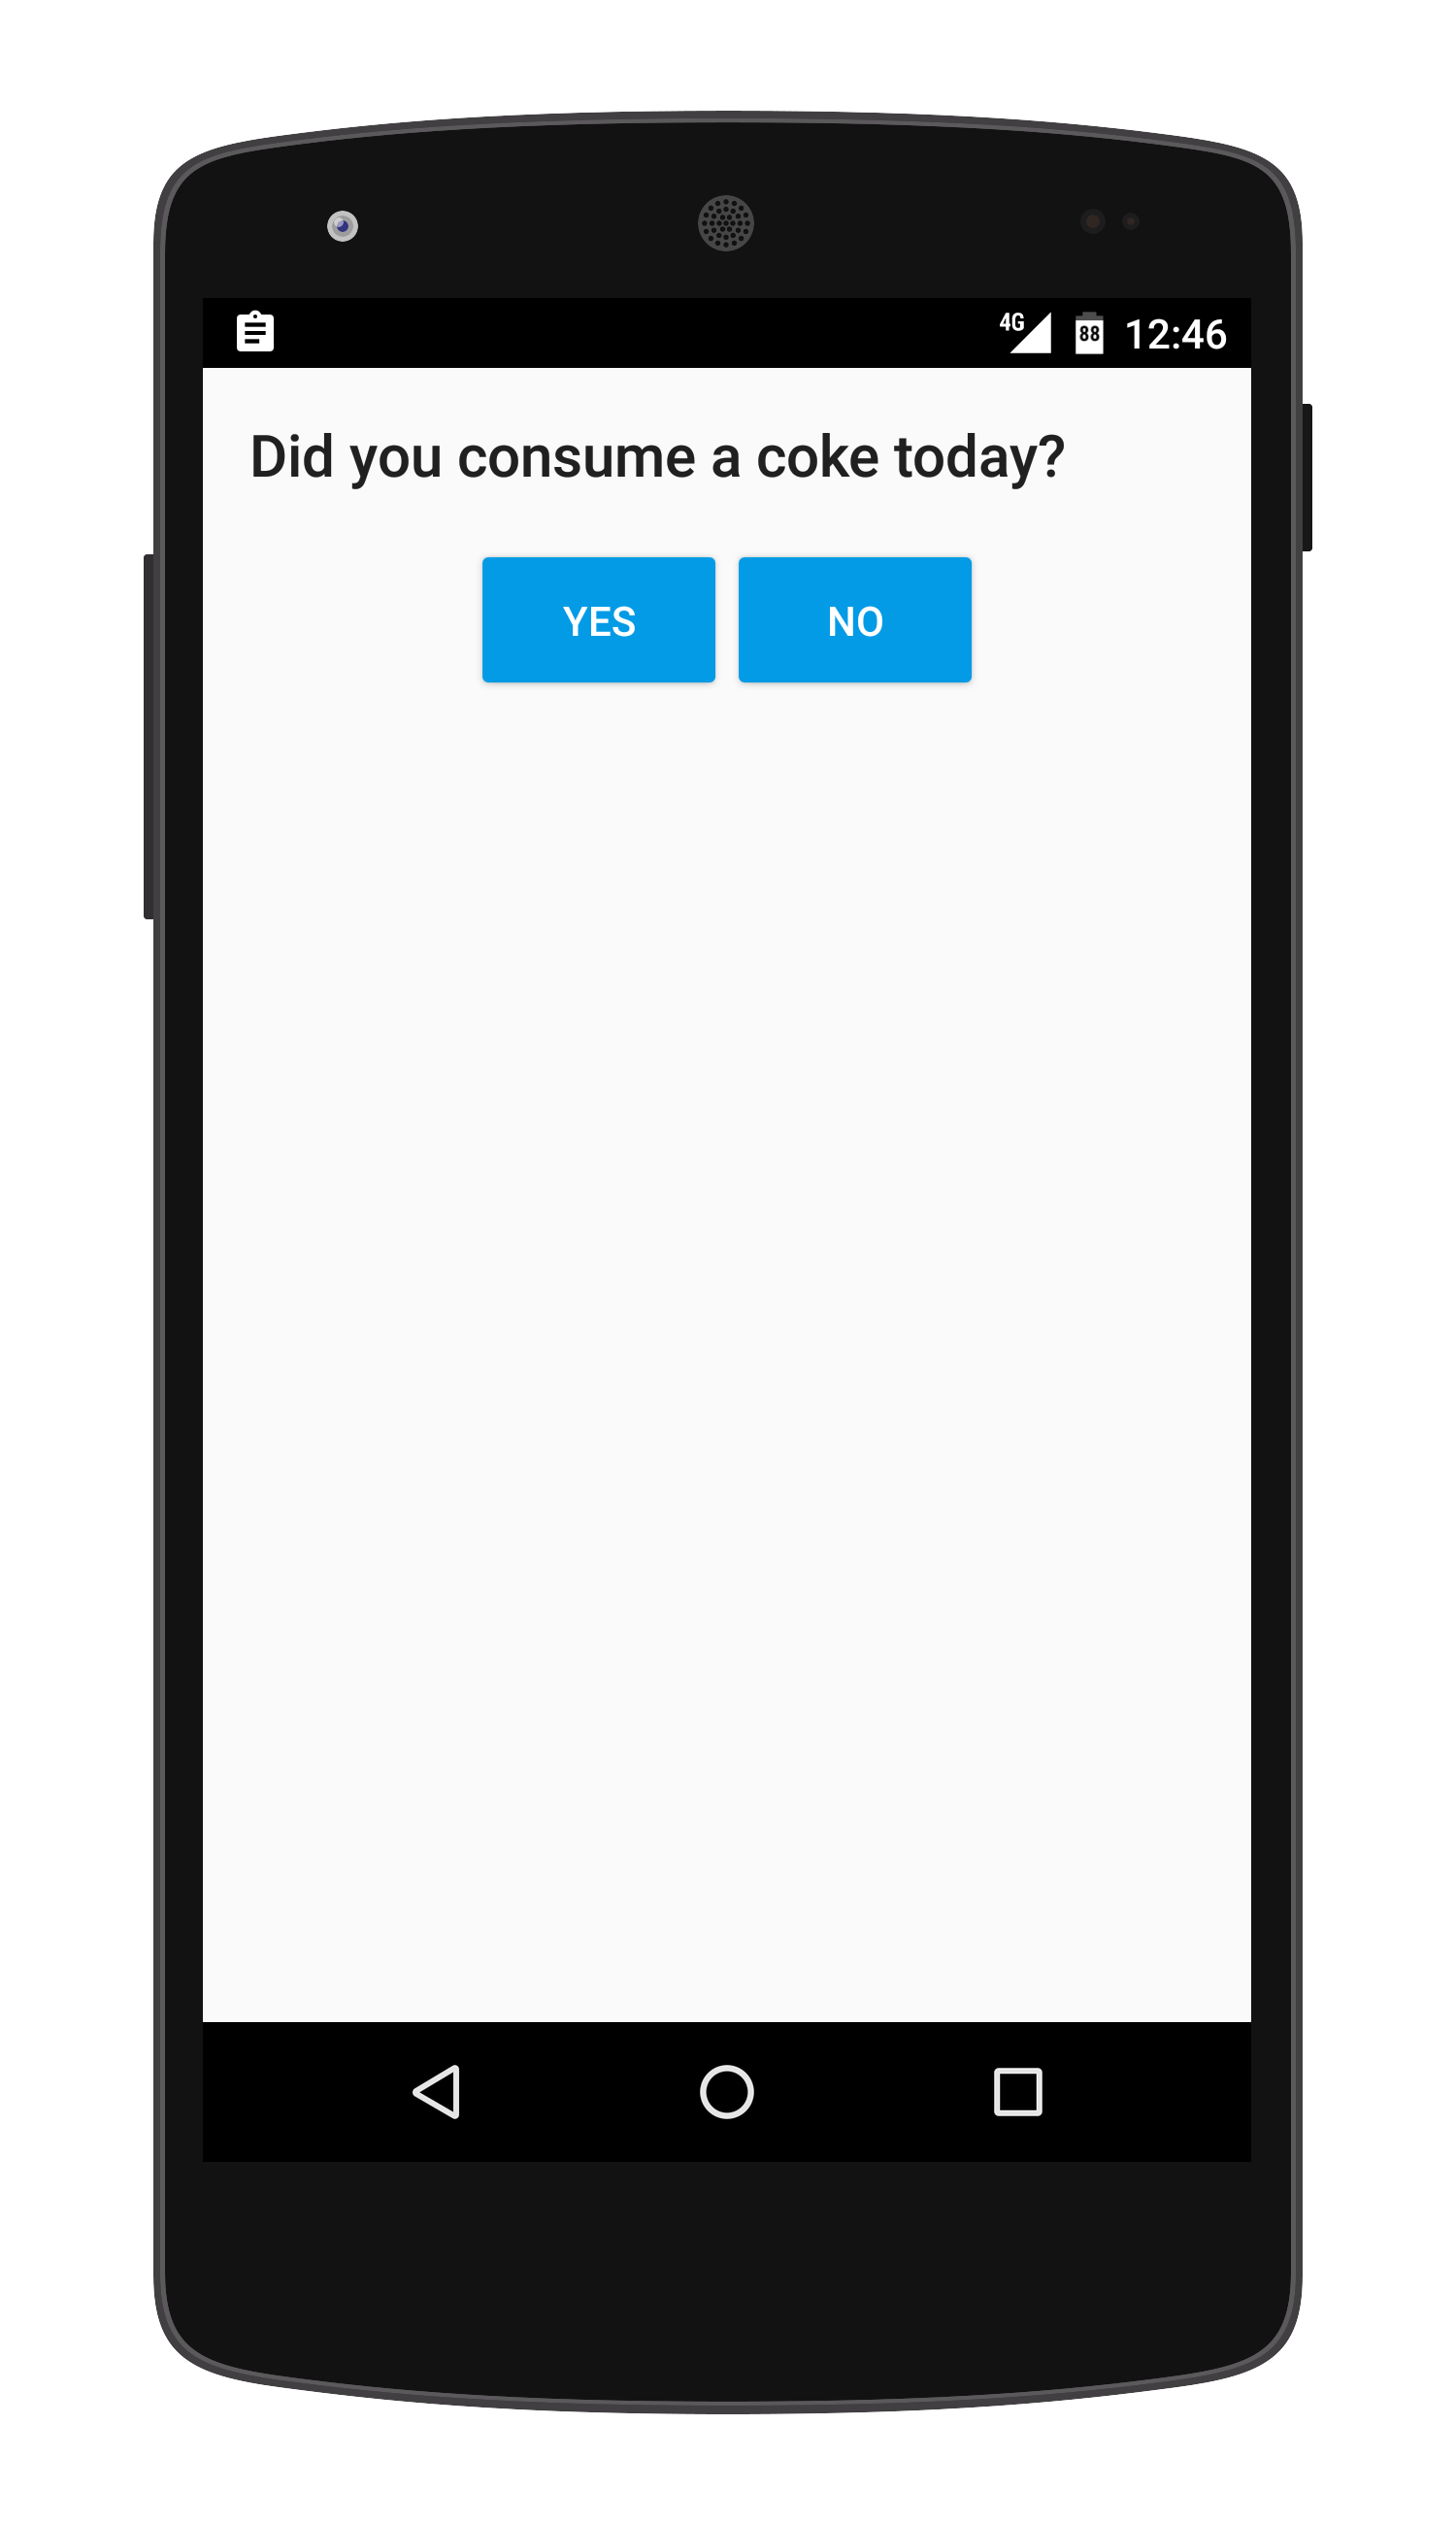
\includegraphics[width=.73\linewidth]{user_interfaces/client/client_answering_questions_with_phone}
  \caption{Answering the questionnaire.}
  \label{fig:answering_questionnaire_answering}
\end{subfigure}
\caption{Notification regarding questionnaire and answer view.}
\label{fig:answering_questionnaire}
\end{figure}
\FloatBarrier